% generated by scripts/make_flow_slides.py from spb_design_flow.tpl.tex; edit the template
\documentclass[aspectratio=169,10pt]{beamer}
\usetheme[progressbar=frametitle,numbering=fraction,block=fill]{metropolis}
\usepackage{booktabs,amsmath,tabularx,multicol}
\usepackage{tikz}
\usepackage[siunitx]{circuitikz}
\usetikzlibrary{arrows.meta,positioning,calc,shapes.geometric}
\definecolor{kth}{RGB}{25,84,166}
\definecolor{kthl}{RGB}{98,152,210}
\definecolor{hs}{RGB}{200,70,50}
\definecolor{ls}{RGB}{50,100,190}
\definecolor{pri}{RGB}{60,140,80}
\setbeamercolor{frametitle}{bg=kth,fg=white}
\setbeamercolor{progress bar}{fg=kthl,bg=kth!20}
\setbeamercolor{title separator}{fg=kthl}
\setbeamercolor{alerted text}{fg=hs}
\graphicspath{{figs/}{../paper/figures/}{../gate-bump/figures/}{../gate-driver/figures/}{../pcb-fab/figures/}{../design-report-v2/figures/}}
\newcommand{\src}[1]{\vfill{\tiny\color{gray}#1}}
% decision box
\newcommand{\decision}[1]{\begin{block}{Decision}#1\end{block}}
% design-flow strip, #1 = active step
\newcommand{\flowstrip}[1]{%
\noindent\resizebox{\linewidth}{!}{\begin{tikzpicture}[font=\tiny,node distance=1.5mm,
  s/.style={draw,rounded corners=1.5pt,minimum height=5mm,text width=15mm,align=center,inner sep=1pt}]
\foreach \k/\t [count=\i] in {1/Inputs,2/Device,3/{Submodule\\voltage},4/{One device,\\one driver},5/{$n$ in\\parallel},6/{$f_\mathrm{sw}$,\\DC link},7/{Gate drive\\$\rightarrow$ block},8/{Two\\blocks},9/{Verify\\block},10/{Rev A\\board}} {
  \ifnum\k=#1 \node[s,fill=kth,text=white] (n\k) at (\i*16.8mm,0) {\t};
  \else \node[s,fill=kth!8] (n\k) at (\i*16.8mm,0) {\t}; \fi}
\foreach \a/\b in {1/2,2/3,3/4,4/5,5/6,6/7,7/8,8/9,9/10} \draw[-{Latex[length=1mm]}] (n\a) -- (n\b);
\end{tikzpicture}}\par\vspace{1mm}}

\title{GaN Building Block for a 1200\,V, 300\,kW Stacked Polyphase Bridge Inverter}
\subtitle{From design inputs to the Rev A board: a decision-driven design}
\author{Enes Ayaz}
\institute{KTH Royal Institute of Technology}
\date{October 2026}

%% numbers from scripts/design_flow_figures.py
\newcommand{\IDEV}{81}
\newcommand{\TRI}{1.8}
\newcommand{\TVF}{5}
\newcommand{\DQ}{0.59}
\newcommand{\CEDGE}{0.4}
\newcommand{\CHO}{2.9}
\newcommand{\FR}{3}
\newcommand{\IOSS}{23}
\newcommand{\IRMS}{228}
\newcommand{\IPK}{322}
\newcommand{\IBLK}{114}
\newcommand{\IPFa}{205}
\newcommand{\IPFb}{216}
\newcommand{\IPFc}{228}
\newcommand{\IPFd}{241}
\newcommand{\RTH}{3.4}
\newcommand{\LCU}{0.31}
\newcommand{\LONE}{0.79}
\newcommand{\LTWO}{0.55}
\newcommand{\LFOUR}{0.43}
\newcommand{\LSIX}{0.39}
\newcommand{\VLeighty}{83}
\newcommand{\ILeighty}{79}
\newcommand{\VLonetwenty}{101}
\newcommand{\ILonetwenty}{119}
\newcommand{\Pb}{33}
\newcommand{\Vb}{131}
\newcommand{\Vc}{96}
\newcommand{\Pc}{22}
\newcommand{\Pd}{18}
\newcommand{\Ph}{15}
\newcommand{\CONDINC}{28}
\newcommand{\ETAtwenty}{99.77}
\newcommand{\ETAfifty}{99.72}
\newcommand{\ETAhundred}{99.63}
\newcommand{\FCROSS}{99}
\newcommand{\NVfifty}{28}
\newcommand{\DVREVA}{4.6}
\newcommand{\FREVA}{57}
\newcommand{\BCOND}{6.2}
\newcommand{\BSW}{2.4}
\newcommand{\BDEAD}{0.3}
\newcommand{\BCU}{5.7}
\newcommand{\BCAP}{0.5}
\newcommand{\BTOT}{15.1}
\newcommand{\BETA}{99.52}
\newcommand{\BPDEV}{2.2}
\newcommand{\BTJ}{67}
\newcommand{\BTOTpfa}{12.5}
\newcommand{\BTOTpfd}{16.7}
\begin{document}
\maketitle

\begin{frame}{Design flow}
\centering
\flowstrip{0}
\vspace{3mm}

\footnotesize
\begin{tabularx}{\linewidth}{@{}clX@{}}
\toprule
1 & Design inputs & 1200\,V, 300\,kW, $M\le1.15$, PMSM $\Rightarrow$ phase current \\
2 & Device & survey 100--650\,V Si/GaN $\Rightarrow$ 100\,V GaN, EPC2361 \\
3 & Submodule voltage & $V_m + L\,di/dt \le 90$\,V with 0.5\,nH, even and integer $N$ $\Rightarrow$ 75\,V, $N=16$ \\
4 & One device, one driver & first-cut loop (copper + MLCC ESL), LTspice: overshoot, energies $\Rightarrow$ $\le$\,80\,A per device \\
5 & Devices in parallel & identical cells: loss, $T_j$ with a realistic $R_\mathrm{th}$, $V_\mathrm{DS}$ vs $n$ $\Rightarrow$ at least 4 per switch \\
6 & $f_\mathrm{sw}$, DC link & losses, MLCC count and current ripple vs $f_\mathrm{sw}$ $\Rightarrow$ 50\,kHz (machine to confirm) \\
7 & Gate drive & one driver for many devices breaks dynamic sharing $\Rightarrow$ one driver per two cells = building block \\
8 & Two blocks & block-to-block sharing and circulating current via the AC connection \\
9--10 & Verification, Rev A & Q3D parasitics, switching, losses, thermal, gate bump, board, measurements \\
\bottomrule
\end{tabularx}
\end{frame}

%==================================================================== 1
\section{1\quad Design inputs}
\begin{frame}{Design inputs}
\flowstrip{1}
\begin{columns}[T]
\column{0.5\textwidth}
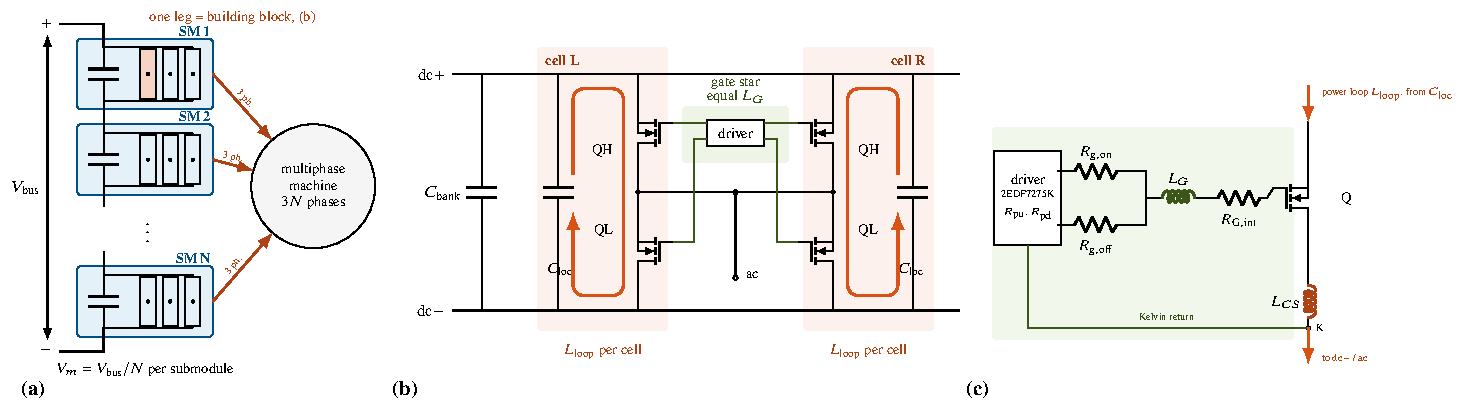
\includegraphics[width=\linewidth]{fig_spb_standalone.pdf}
\column{0.48\textwidth}
\small
\begin{tabular}{@{}ll@{}}
\toprule
DC bus & 1200\,V nominal \\
Output power & 300\,kW \\
Modulation index & $M \le 1.15$ (SVM) \\
Machine & PMSM, $\cos\varphi$ assumed 0.9 \\
Switching frequency & open (20--100\,kHz), step 6 \\
Coolant & 60\,$^\circ$C, $T_j \le 125\,^\circ$C \\
Device stress & $V_\mathrm{DS} \le 90$\,V at nominal bus (100\,V part) \\
\bottomrule
\end{tabular}

\vspace{1ex}
\footnotesize SPB: $N$ three-phase submodules in series on the DC side, each feeding one winding set; $V_m = 1200\,\mathrm{V}/N$.
\end{columns}
\end{frame}

\begin{frame}{Phase current follows from the inputs}
\flowstrip{1}
\vspace{1mm}
\begin{columns}[T]
\column{0.55\textwidth}
\small
Each of the $3N$ legs delivers $P/3N$ at the rms phase voltage $V_\mathrm{ph}=M V_m/(2\sqrt2)$:
\[
I_\mathrm{rms} = \frac{P}{3N\,V_\mathrm{ph}\cos\varphi}
 = \frac{P}{3\,\dfrac{M\,V_\mathrm{bus}}{2\sqrt2}\cos\varphi}
\]
\begin{itemize}
\item $N V_m = V_\mathrm{bus}$: the phase current does \alert{not} depend on $N$
\item $V_\mathrm{ph}$ = 1.15 $\cdot$ 75\,V/$2\sqrt2$ = 30.5\,V; 6.25\,kW per leg
\item \textbf{\IRMS\,A$_\mathrm{rms}$ per leg}, \IPK\,A peak ($\cos\varphi$ = 0.9)
\end{itemize}
\column{0.43\textwidth}
\small
\begin{tabular}{@{}cc@{}}
\toprule
$\cos\varphi$ & $I_\mathrm{rms}$ per leg \\
\midrule
1.00 & \IPFa\,A \\
0.95 & \IPFb\,A \\
0.90 & \textbf{\IPFc\,A} \\
0.85 & \IPFd\,A \\
\bottomrule
\end{tabular}

\vspace{1ex}
\footnotesize Losses below are for $\cos\varphi$ = 0.9; the PMSM operating point (field weakening, $\cos\varphi$) must be confirmed with the machine design.
\end{columns}
\end{frame}

%==================================================================== 2
\section{2\quad Device}
\begin{frame}{Voltage class: why 100\,V GaN}
\begin{columns}[T]
\column{0.6\textwidth}
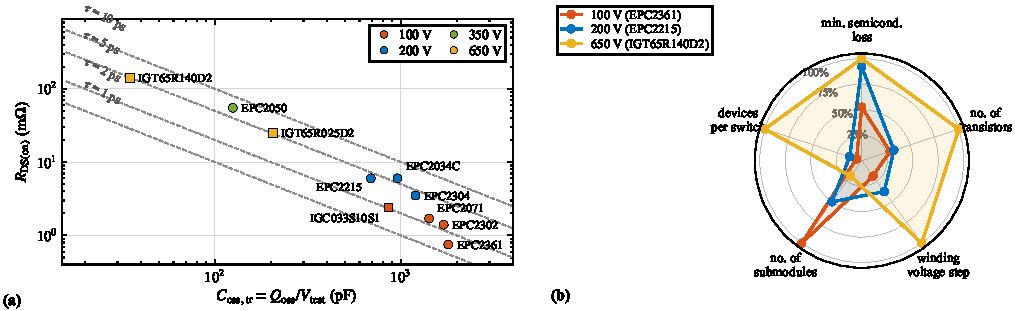
\includegraphics[width=\linewidth]{fig_devices.pdf}
\column{0.38\textwidth}
\small
\begin{itemize}
\item At fixed bus voltage and phase current the minimum semiconductor loss scales with the device time constant $R_\mathrm{DS(on)}C_\mathrm{oss,tr}$
\item 100\,V GaN gives the lowest product among 100--650\,V Si/SiC/GaN candidates
\item Selected: \textbf{EPC2361}, 100\,V, 0.75\,m$\Omega$ typ, 3\,$\times$\,5\,mm, top-side cooling
\end{itemize}
\end{columns}
\end{frame}
\begin{frame}{EPC2361 key data}
\begin{columns}[T]
\column{0.55\textwidth}
\small
\begin{tabular}{@{}ll@{}}
\toprule
$V_\mathrm{DS}$ / transient & 100 / 120\,V \\
$R_\mathrm{DS(on)}$ & 0.75\,m$\Omega$ typ (1.0 max) \\
$V_\mathrm{GS}$ range & $-4$ \dots\ $+6$\,V \\
$V_\mathrm{GS(th)}$ & 0.8 / 1.1 / 2.5\,V \\
$C_\mathrm{iss}$ / $C_\mathrm{oss}$ / $C_\mathrm{rss}$ & 3599 / 1019 / 13\,pF \\
$Q_G$ / $Q_{GD}$ / $Q_\mathrm{OSS}$ & 28 / 3.8 / 90\,nC \\
$R_\mathrm{G,int}$ & 0.4\,$\Omega$ \\
$R_{\theta\mathrm{JC}}$ top / $R_{\theta\mathrm{JB}}$ & 0.2 / 1.5\,K/W \\
\bottomrule
\end{tabular}
\column{0.43\textwidth}
\small
\begin{itemize}
\item Low threshold and $-4$\,V limit: gate drive needs care (bump, negative bias)
\item Top of the package at \alert{source potential}: thermal interface must insulate
\item Seven interleaved stripes, pad 2 next to the gate is the natural Kelvin point
\end{itemize}
\end{columns}
\end{frame}
%==================================================================== 3
\section{3\quad Submodule voltage}
\begin{frame}{Submodule voltage from $L\,di/dt$}
\flowstrip{3}
\begin{columns}[T]
\column{0.54\textwidth}
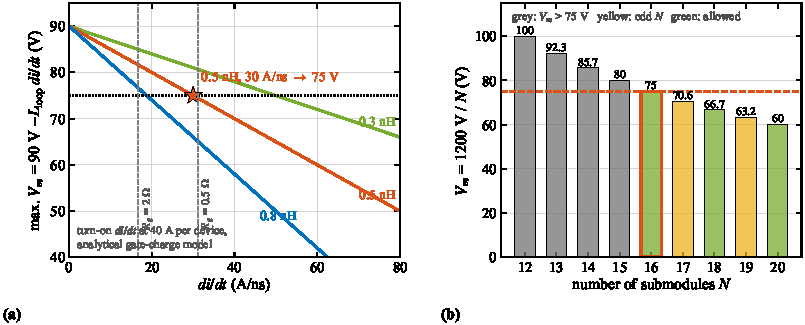
\includegraphics[width=\linewidth]{flow_vm.pdf}
\column{0.44\textwidth}
\scriptsize
\begin{itemize}
\item Peak stress $\hat v_\mathrm{DS} = V_m + L_\mathrm{loop}\,di/dt \le 90$\,V (10\,\% below the 100\,V rating)
\item First-cut loop with MLCCs: $L_\mathrm{loop}\approx$\,0.5\,nH per cell
\item To use the device fully we want fast switching: $\approx$\,30\,A/ns (analytical gate-charge model, 40\,A per device, $R_g$ 0.5--2\,$\Omega$) $\Rightarrow$ 15\,V overshoot
\item $\Rightarrow$ $V_m \le 75$\,V
\item $N$ must be an integer and even (symmetric arrangement of submodules and winding sets): 14 cells give 86\,V, 18 cells 67\,V and 12.5\,\% more parts
\end{itemize}
\decision{$V_m$ = 75\,V, $N$ = 16}
\end{columns}
\end{frame}

\begin{frame}{Why not lower: every submodule costs parts and loss}
\flowstrip{3}
\begin{columns}[T]
\column{0.5\textwidth}
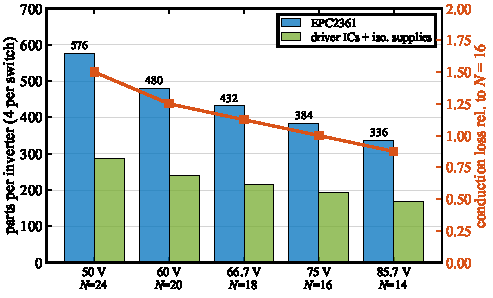
\includegraphics[width=\linewidth]{flow_cells.pdf}
\column{0.48\textwidth}
\small
\begin{itemize}
\item Phase current is fixed by $P$, $V_\mathrm{bus}$, $M$, $\cos\varphi$, not by $N$
\item Each submodule carries the full phase current $\Rightarrow$ conduction loss, transistors, drivers and isolated supplies all scale with $N$
\item 60\,V ($N$ = 20): +25\,\% parts and conduction loss
\item At the maximum bus voltage the overshoot margin shrinks; checked with the final Rev B layout (Q3D: 0.41\,nH per cell on the load board, 0.65\,nH on the DPT board with the shunt)
\end{itemize}
\end{columns}
\end{frame}

%==================================================================== 4
\section{4\quad One device, one driver}
\begin{frame}{First-cut power loop of one cell}
\flowstrip{4}
\begin{columns}[T]
\column{0.54\textwidth}
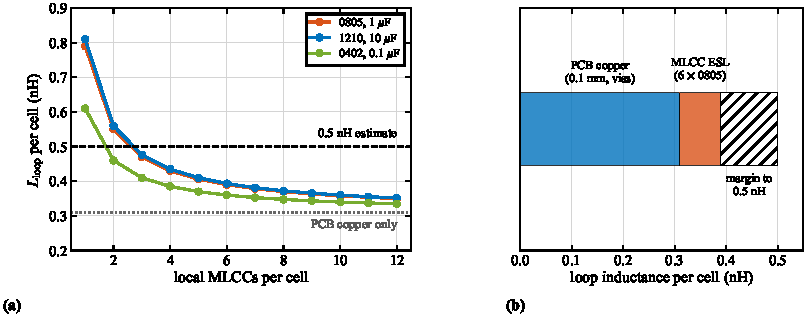
\includegraphics[width=\linewidth]{flow_loop.pdf}
\column{0.44\textwidth}
\scriptsize
\begin{itemize}
\item Loop = PCB copper (vertical loop over a 0.1\,mm dielectric, vias, pads) + ESL of the local MLCCs; the LGA package is in the device model
\item Copper alone $\approx$\,\LCU\,nH; MLCCs in parallel add ESL/$n_c$
\item 1 / 2 / 4 / 6 MLCCs: \LONE\ / \LTWO\ / \LFOUR\ / \LSIX\,nH: beyond $\approx$\,4 the number hardly matters
\item Chosen part: 1\,\textmu F 100\,V X7S 0805 (TDK C2012X7S2A105K125AB), next to the drains
\end{itemize}
\decision{Design with $L_\mathrm{loop}$ = 0.5\,nH per cell (0.3 and 0.8\,nH as bounds)}
\end{columns}
\end{frame}

\begin{frame}{One EPC2361 per switch: how fast and how much overshoot}
\flowstrip{4}
\centering
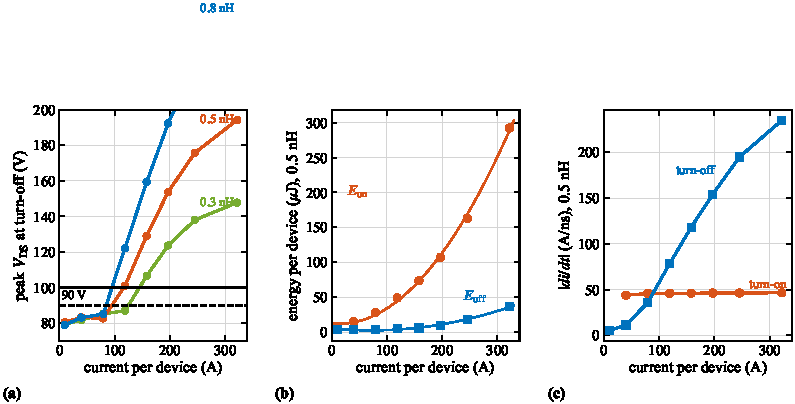
\includegraphics[width=\linewidth,height=0.37\textheight,keepaspectratio]{flow_single.pdf}
\footnotesize
\begin{itemize}
\item LTspice half bridge, double pulse at 75\,V: lumped loop, 1.7\,nH gate loop, 0.03\,nH common source, 2\,$\Omega$ on / 0\,$\Omega$ off, 4\,A/8\,A driver
\item Turn-on $di/dt$ is set by the driver ($\approx$\,45\,A/ns); turn-off $di/dt$ grows with current as the output capacitance charges faster
\item 0.5\,nH: \VLeighty\,V at \ILeighty\,A, \alert{\VLonetwenty\,V at \ILonetwenty\,A} per device; $E_\mathrm{on}$ grows quadratically
\item One device would carry \IPK\,A peak $\Rightarrow$ \textbf{current per device must stay $\le$\,80\,A}
\end{itemize}
\end{frame}

%==================================================================== 5
\section{5\quad Devices in parallel}
\begin{frame}{Thermal path per device}
\flowstrip{5}
\begin{columns}[T]
\column{0.55\textwidth}
\small
\begin{tabular}{@{}lr@{}}
\toprule
Layer (top-side cooling, per device) & K/W \\
\midrule
$R_{\theta JC}$ (top), datasheet & 0.20 \\
TIM 1, 50 $\mu$m, 3 W/mK, 15 mm$^2$ & 1.11 \\
AlN 0.635 mm, 170 W/mK, 25 mm$^2$ & 0.15 \\
TIM 2, 50 $\mu$m, 3 W/mK, 50 mm$^2$ & 0.33 \\
cold plate, $h$ = 10 kW/m$^2$K, 100 mm$^2$ & 1.00 \\
coupling to neighbours, coolant rise (+20 \%) & 0.56 \\
\midrule
Junction--coolant & \textbf{\RTH} \\
\bottomrule
\end{tabular}
\column{0.43\textwidth}
\small
\begin{itemize}
\item The earlier 2.1\,K/W was optimistic: two TIM layers and the cold plate dominate
\item Used for the decisions: \textbf{\RTH\,K/W}, coolant 60\,$^\circ$C
\item Bounds: 2.1\,K/W (sintered/soldered stack) and 8\,K/W (gap pad, as on the lab board)
\item $R_\mathrm{DS(on)}(T_j)$ from the datasheet curve (1.49 at 100\,$^\circ$C, 1.80 at 150\,$^\circ$C)
\end{itemize}
\end{columns}
\end{frame}

\begin{frame}{$n$ identical cells per switch (one device and one driver each)}
\flowstrip{5}
\centering
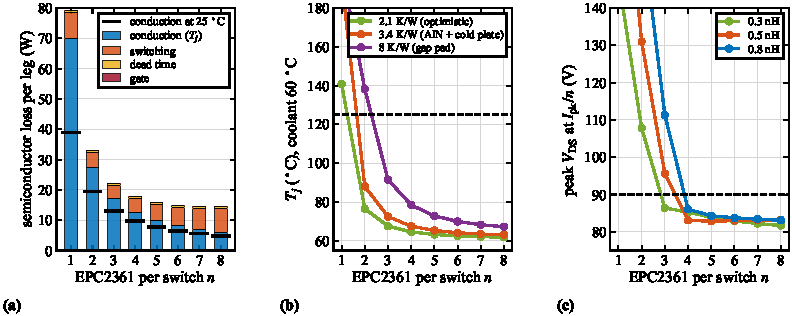
\includegraphics[width=\linewidth,height=0.42\textheight,keepaspectratio]{flow_npar.pdf}
\footnotesize
\begin{itemize}
\item \IRMS\,A$_\mathrm{rms}$ per leg, 50\,kHz, $T_j$ and $R_\mathrm{DS(on)}$ solved together; LTspice energies at 0.5\,nH
\item $n$ = 1: $T_j$ beyond 150\,$^\circ$C; $n$ = 2: \Pb\,W and \Vb\,V; $n$ = 3: \Vc\,V at 0.5\,nH
\item $n$ = 4 / 8: \Pd\,/\,\Ph\,W per leg; above 4 the gain is small while $E_\mathrm{oss}$ and drivers grow
\end{itemize}
\vspace{-1ex}
\decision{At least \textbf{4 EPC2361 per switch} ($V_\mathrm{DS}$ and $T_j$ for all three $R_\mathrm{th}$; 4 also splits into two equal pairs)}
\end{frame}

\begin{frame}{Where the loss comes from: line period and junction temperature}
\flowstrip{5}
\centering
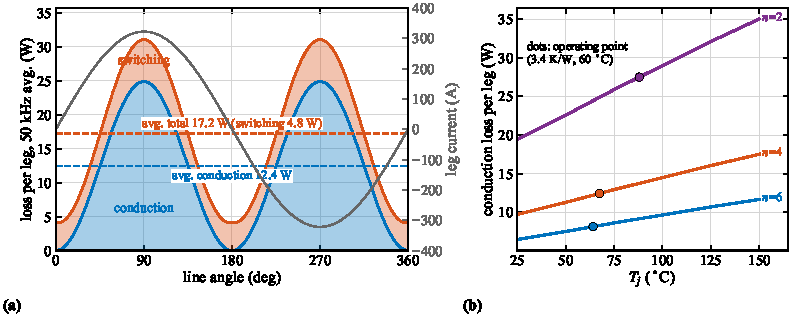
\includegraphics[width=\linewidth,height=0.48\textheight,keepaspectratio]{flow_wave.pdf}
\footnotesize
\begin{itemize}
\item $n$ = 4, 50\,kHz: switching loss follows $|i|$ (plus a constant $E_\mathrm{oss}$ part), conduction loss follows $i^2$; both peak at the current maximum
\item Conduction loss at the operating point is \CONDINC\,\% above its 25\,$^\circ$C value; with $n$ = 2 the self-heating loop ($T_j\uparrow\Rightarrow R_\mathrm{DS(on)}\uparrow$) is much stronger
\end{itemize}
\end{frame}

\begin{frame}{Losses vs number in parallel}
\flowstrip{5}
\footnotesize
\begin{tabular}{@{}lrrrrrrrr@{}}
\toprule
$n$ per switch & 1 & 2 & 3 & 4 & 5 & 6 & 7 & 8 \\
\midrule
Loss per leg (W) & 79.1 & 33.0 & 22.1 & 17.8 & 15.8 & 14.9 & 14.5 & 14.5 \\
\quad conduction at $T_j$ (W) & 70.0 & 27.5 & 17.0 & 12.4 & 9.8 & 8.1 & 7.0 & 6.1 \\
\quad conduction at 25\,$^\circ$C (W) & 38.9 & 19.4 & 13.0 & 9.7 & 7.8 & 6.5 & 5.6 & 4.9 \\
\quad switching (W) & 8.4 & 5.0 & 4.5 & 4.8 & 5.4 & 6.2 & 7.0 & 7.9 \\
Efficiency (\%) & 98.73 & 99.47 & 99.65 & 99.72 & 99.75 & 99.76 & 99.77 & 99.77 \\
Loss per device (W) & 39.5 & 8.2 & 3.7 & 2.2 & 1.6 & 1.2 & 1.0 & 0.9 \\
$T_j$ ($^\circ$C) & 194 & 88 & 72 & 68 & 65 & 64 & 63 & 63 \\
Peak $V_\mathrm{DS}$ (V) & \alert{194} & \alert{131} & \alert{96} & 83 & 83 & 83 & 83 & 83 \\
Driver channels per leg & 2 & 4 & 6 & 8 & 10 & 12 & 14 & 16 \\
\bottomrule
\end{tabular}

\vspace{1ex}
\footnotesize Semiconductor losses only (conduction at $T_j$, switching incl.\ $E_\mathrm{oss}$, dead time, gate), \RTH\,K/W, 60\,$^\circ$C coolant, 0.5\,nH, 50\,kHz. Board copper and MLCC losses are added for the block on the verification slides. Efficiency relative to 6.25\,kW per leg.
\end{frame}

%==================================================================== 6
\section{6\quad Switching frequency and DC link}
\begin{frame}{Switching frequency: losses, DC-link capacitors, current ripple}
\flowstrip{6}
\centering
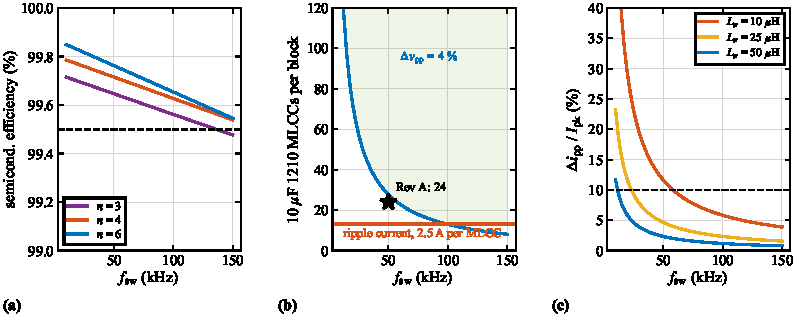
\includegraphics[width=\linewidth,height=0.34\textheight,keepaspectratio]{flow_fsw.pdf}
\scriptsize
\begin{itemize}
\item (a) $n$ = 4: \ETAtwenty\,/\,\ETAfifty\,/\,\ETAhundred\,\% at 20 / 50 / 100\,kHz
\item (b) DC link per block (\IBLK\,A$_\mathrm{rms}$, 4\,\% ripple, 10\,\textmu F 1210 at 30\,\% of $C$ at 75\,V): voltage ripple sets the count below $\approx$\,\FCROSS\,kHz, ripple current above; at 50\,kHz $\approx$\,\NVfifty\ MLCCs
\item (c) Winding current ripple $\Delta i_\mathrm{pp} = V_m/(4L_\sigma f_\mathrm{sw})$ depends on the machine leakage inductance $L_\sigma$ (not known yet)
\end{itemize}
\vspace{-1ex}
\decision{$f_\mathrm{sw}$ = 50\,kHz for the block design (efficiency and capacitor count balanced); final value with the machine ($L_\sigma$, iron loss)}
\end{frame}

\begin{frame}{Bypass capacitors: how many and how large}
\flowstrip{6}
\begin{columns}[T]
\column{0.44\textwidth}
\vspace{2mm}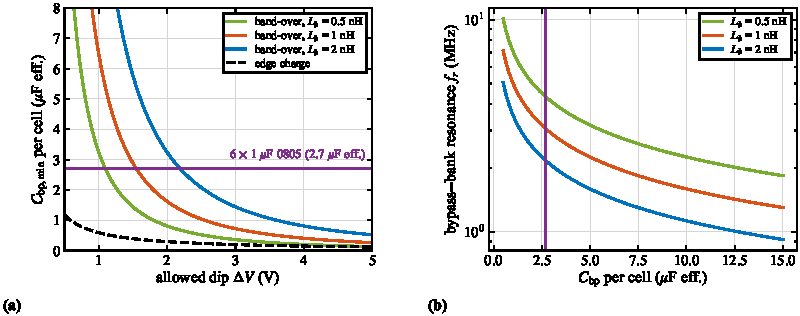
\includegraphics[width=\linewidth]{flow_bypass.pdf}
\column{0.54\textwidth}
\scriptsize
\textbf{Bypass} (1\,\textmu F 0805) supplies the edge, \textbf{bank} (10\,\textmu F 1210) the $f_\mathrm{sw}$ ripple. Per cell, \IDEV\,A:
\begin{enumerate}\setlength\itemsep{0pt}
\item \textbf{$di/dt$ $\rightarrow$ number}: $L_\mathrm{loop} = L_\mathrm{Cu} + \mathrm{ESL}/n \le 0.5$\,nH $\Rightarrow n \ge 4$
\item \textbf{Edge charge}: $\Delta Q = I(t_{ri}/2 + t_{vf}) + Q_\mathrm{oss}$, $t_{ri} = I/(di/dt)$ = \TRI\,ns, $t_{vf} = V/(dv/dt)$ = \TVF\,ns: \DQ\,\textmu C $\Rightarrow$ \CEDGE\,\textmu F for 1.5\,V ($C_\mathrm{oss}\,dv/dt$ = \IOSS\,A is included in $Q_\mathrm{oss}$)
\item \textbf{Hand-over to the bank} through $L_b$: $\Delta V \approx \Delta I\sqrt{L_b/C_\mathrm{bp}}$ $\Rightarrow$ $C_\mathrm{bp} \ge L_b(\Delta I/\Delta V)^2$ = \CHO\,\textmu F (1\,nH, 1.5\,V): \alert{sets the capacitance}
\item \textbf{Checks}: $C_\mathrm{bp} \gg C_\mathrm{oss}$ ($\ge$\,20$\times$); bypass--bank resonance $f_r$ = \FR\,MHz is excited every edge, damped only by ESR $\Rightarrow$ no more bypass than needed, $C_\mathrm{bank} \ge 10\,C_\mathrm{bp}$; X7S at 75\,V keeps 45\,\%
\end{enumerate}
\decision{6 $\times$ 1\,\textmu F 0805 per cell (2.7\,\textmu F eff.); $L_b$ to be extracted with Q3D on the routed board}
\end{columns}
\end{frame}

\begin{frame}{DC-link capacitor selection}
\flowstrip{6}
\begin{columns}[T]
\column{0.55\textwidth}
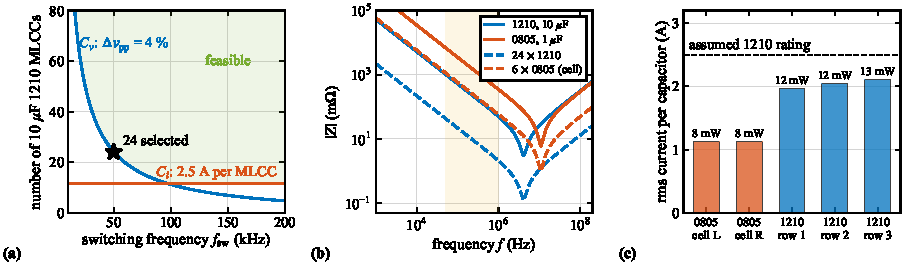
\includegraphics[width=\linewidth]{fig_dclink.pdf}
\column{0.43\textwidth}
\footnotesize
\begin{itemize}
\item Local: 6\,$\times$ 1\,\textmu F 0805 per cell (loop inductance, slide 4); bank: 10\,\textmu F 100\,V X7S 1210 (Murata GRM32EC72A106KE05L)
\item $C$ at 75\,V only $\approx$\,30\,\% of nominal (X7S DC bias)
\item Rev A has 24 per block, sized for 100\,A$_\mathrm{rms}$; at \IBLK\,A and 50\,kHz the ripple is $\approx$\,\DVREVA\,\% (4\,\% from \FREVA\,kHz), or add MLCCs in Rev B
\item Loss $\approx$\,0.4--0.5\,W per block; ripple current $\approx$\,2\,A per part
\end{itemize}
\end{columns}
\end{frame}
%==================================================================== 6
\section{7\quad Gate drive: from 4 devices to a building block}
\begin{frame}{Can one driver drive all four?}
\flowstrip{7}
\begin{columns}[T]
\column{0.58\textwidth}
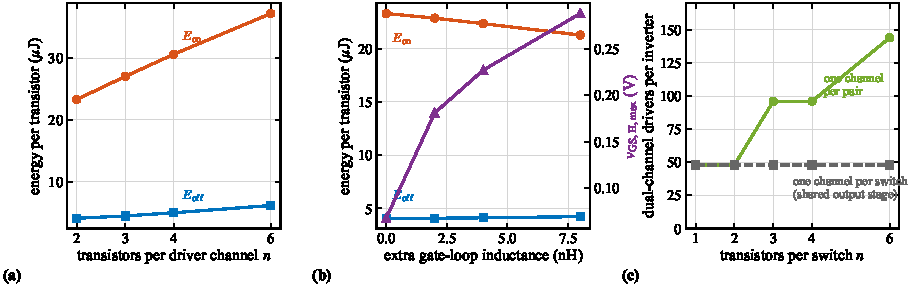
\includegraphics[width=\linewidth]{drv_scaling.pdf}
\column{0.4\textwidth}
\small
\begin{itemize}
\item One channel for 3 / 4 / 6 transistors: $E_\mathrm{on}$ per transistor $+16$ / $+31$ / $+60$\,\%
\item Peak sink current 12--14\,A, above the 8\,A rating
\item Longer gate tree brings the gate bump back
\item One driver per device: symmetric, but 4 channels and isolated supplies per switch
\end{itemize}
\end{columns}
\end{frame}
\begin{frame}{Why symmetry: current-sharing sensitivity}
\begin{columns}[T]
\column{0.6\textwidth}
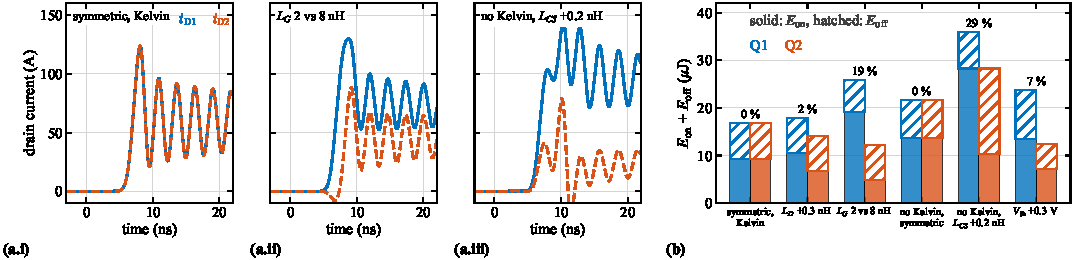
\includegraphics[width=\linewidth]{fig_sharing.pdf}
\column{0.38\textwidth}
\small
\begin{itemize}
\item Static sharing is fine ($R_\mathrm{DS(on)}$ has positive TC)
\item Dynamic sharing is set by the gate circuits:
\begin{itemize}\footnotesize
\item gate-loop mismatch 2 vs 8\,nH $\rightarrow$ 19\,\% imbalance, 4:1 $E_\mathrm{on}$
\item common-source mismatch without Kelvin $\rightarrow$ 29\,\%, $2.8\times E_\mathrm{on}$ in one device
\end{itemize}
\item $\Rightarrow$ star-connected gate drive with Kelvin returns, one driver channel per pair
\end{itemize}
\end{columns}
\end{frame}
\begin{frame}{Kelvin source on the EPC2361}
\begin{columns}[T]
\column{0.52\textwidth}
\centering
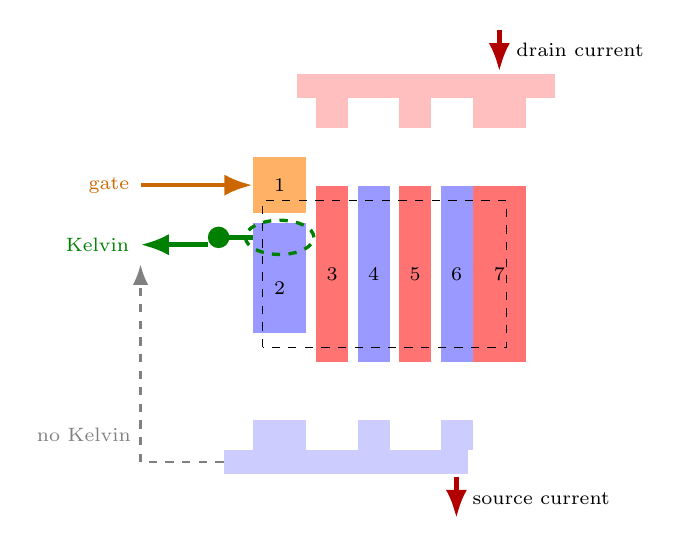
\begin{tikzpicture}[scale=0.62]
% drain / source copper
\fill[red!25] (1.0,3.6) rectangle (6.3,4.1);
\foreach \x/\w in {1.725/0.65,3.425/0.65,5.152/1.10} \fill[red!25] (\x-\w/2,3.0) rectangle (\x+\w/2,3.6);
\fill[blue!20] (-0.5,-4.1) rectangle (4.5,-3.6);
\foreach \x/\w in {0.648/1.10,2.575/0.65,4.275/0.65} \fill[blue!20] (\x-\w/2,-3.6) rectangle (\x+\w/2,-3.0);
% pads
\fill[orange!60] (0.097,1.25) rectangle (1.199,2.39);
\fill[blue!40] (0.097,-1.21) rectangle (1.199,1.05);
\foreach \x in {1.725,3.425} \fill[red!55] (\x-0.325,-1.8) rectangle (\x+0.325,1.8);
\foreach \x in {2.575,4.275} \fill[blue!40] (\x-0.325,-1.8) rectangle (\x+0.325,1.8);
\fill[red!55] (4.601,-1.8) rectangle (5.703,1.8);
\draw[dashed] (0.3,-1.5) rectangle (5.3,1.5);
\node at (0.65,1.82) {\scriptsize 1};
\node at (0.65,-0.3) {\scriptsize 2};
\foreach \x/\n in {1.725/3,2.575/4,3.425/5,4.275/6,5.152/7} \node at (\x,0) {\scriptsize \n};
% Kelvin
\draw[green!50!black,line width=1.2pt,dashed] (0.65,0.75) ellipse (0.7 and 0.35);
\fill[green!50!black] (-0.6,0.75) circle (0.22);
\draw[green!50!black,line width=1.6pt] (0.097,0.75) -- (-0.38,0.75);
\draw[green!50!black,line width=1.6pt,-{Latex}] (-0.82,0.6) -- (-2.2,0.6) node[left]{\scriptsize Kelvin};
\draw[orange!80!black,line width=1.6pt,{Latex}-] (0.097,1.82) -- (-2.2,1.82) node[left]{\scriptsize gate};
\draw[gray,line width=1pt,dashed,-{Latex}] (-0.5,-3.85) -- (-2.2,-3.85) -- (-2.2,0.2);
\node[gray,left] at (-2.2,-3.3) {\scriptsize no Kelvin};
\draw[red!70!black,line width=1.6pt,-{Latex}] (5.15,5.0) -- (5.15,4.15);
\draw[red!70!black,line width=1.6pt,-{Latex}] (4.27,-4.15) -- (4.27,-5.0);
\node[right] at (5.3,4.6) {\scriptsize drain current};
\node[right] at (4.4,-4.6) {\scriptsize source current};
\end{tikzpicture}
\column{0.46\textwidth}
\small
\begin{itemize}
\item Pad 2 is a separate source pad next to the gate pad; its gate end carries almost no load current
\item Kelvin via at that end; return routed to the driver on its own path (L2 / L4)
\item Gate loop (horizontal) $\perp$ power loop (vertical): minimum coupling
\item Q3D: $L_{CS}$ = \textbf{0.030\,nH} with Kelvin, 0.061\,nH without $\Rightarrow$ $\approx$\,0.5 vs 1.0\,V subtracted from $V_{GS}$ at 17\,A/ns
\end{itemize}
\end{columns}
\end{frame}
\begin{frame}{Building block: two point-symmetric cells, one centre driver}
\flowstrip{7}
\begin{columns}[T]
\column{0.5\textwidth}
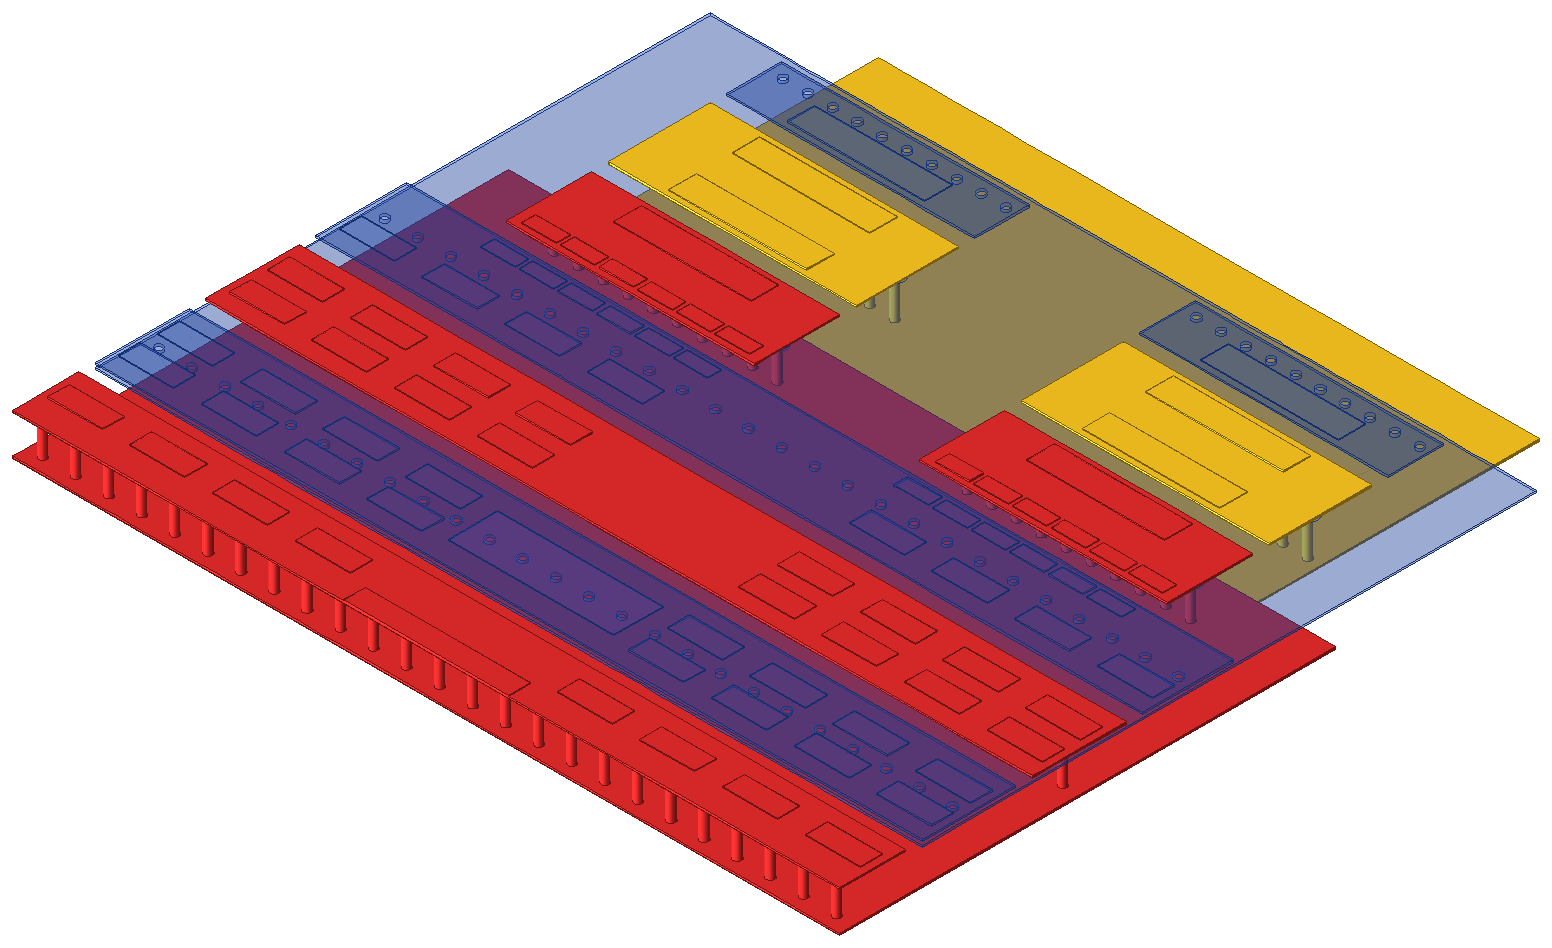
\includegraphics[width=\linewidth]{q3d_model.png}
\column{0.48\textwidth}
\small
\begin{itemize}
\item Two cells rotated by 180$^\circ$ about the driver (point symmetry): identical gate loops and Kelvin returns for both transistors of a switch
\item One 2EDF7275K channel drives a \textbf{pair} symmetrically (star gate network)
\item Each cell keeps its own commutation loop (Rev B, Q3D: 0.41\,nH per cell, load board)
\end{itemize}
\decision{Building block = 2\,$\times$ EPC2361 per switch, one driver; \textbf{4 per switch = two blocks}}
\end{columns}
\end{frame}

%==================================================================== 7
\section{8\quad Two blocks in parallel}
\begin{frame}{Two building blocks per leg}
\flowstrip{8}
\begin{columns}[T]
\column{0.54\textwidth}
\centering
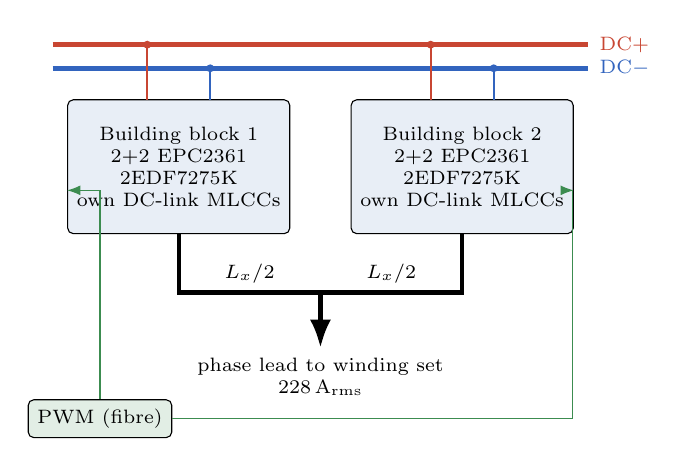
\begin{tikzpicture}[font=\scriptsize,
  blk/.style={draw,rounded corners=2pt,fill=kth!10,minimum width=24mm,minimum height=17mm,align=center}]
\node[blk] (a) at (0,0) {Building block 1\\2+2 EPC2361\\2EDF7275K\\own DC-link MLCCs};
\node[blk] (b) at (3.6,0) {Building block 2\\2+2 EPC2361\\2EDF7275K\\own DC-link MLCCs};
\draw[hs,line width=1.6pt] (-1.6,1.55) -- (5.2,1.55) node[right]{DC$+$};
\draw[ls,line width=1.6pt] (-1.6,1.25) -- (5.2,1.25) node[right]{DC$-$};
\foreach \x in {-0.4,3.2} {\draw[hs,thick] (\x,1.55) -- (\x,0.85); \fill[hs] (\x,1.55) circle (0.05);}
\foreach \x in {0.4,4.0} {\draw[ls,thick] (\x,1.25) -- (\x,0.85); \fill[ls] (\x,1.25) circle (0.05);}
\draw[line width=1.6pt] (0,-0.85) -- (0,-1.6) -- (3.6,-1.6) -- (3.6,-0.85);
\draw[line width=1.6pt,-{Latex}] (1.8,-1.6) -- (1.8,-2.3);
\node[below,align=center] at (1.8,-2.3) {phase lead to winding set\\\IRMS\,A$_\mathrm{rms}$};
\node[above] at (0.9,-1.6) {$L_x/2$};
\node[above] at (2.7,-1.6) {$L_x/2$};
\node[draw,fill=pri!15,rounded corners=2pt] (f) at (-1.0,-3.2) {PWM (fibre)};
\draw[pri,-{Latex}] (f.north) -- (-1.0,-0.3) -- (a.west|- 0,-0.3);
\draw[pri,-{Latex}] (f.east) -- (5.0,-3.2) -- (5.0,-0.3) -- (b.east|- 0,-0.3);
\end{tikzpicture}
\column{0.44\textwidth}
\small
\begin{itemize}
\item Two unchanged blocks share the submodule DC link and are joined at the AC side
\item Per block \IBLK\,A$_\mathrm{rms}$ (\IRMS\,A per leg)
\item Commutation stays inside each block (own MLCCs)
\item System: 96 blocks, 96 drivers, 384 EPC2361; series DC chain carries 250\,A
\end{itemize}
\end{columns}
\end{frame}

\begin{frame}{Sharing between blocks: driver skew and the AC connection}
\flowstrip{8}
\centering
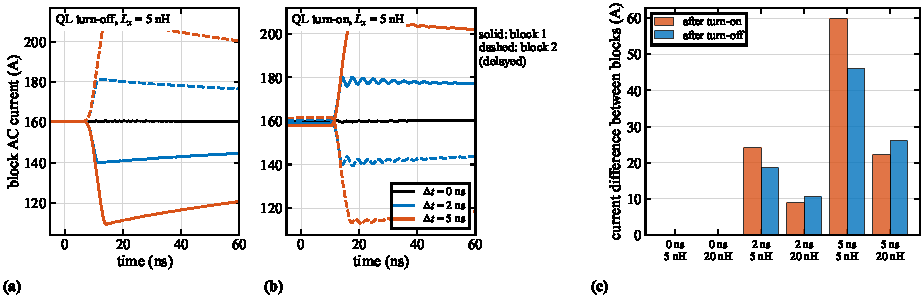
\includegraphics[width=\linewidth,height=0.40\textheight,keepaspectratio]{flow_twoblock.pdf}
\footnotesize
\begin{itemize}
\item LTspice, two complete blocks at \IPK\,A, PWM of block 2 delayed by $\Delta t$; $L_x$ = AC inductance between the switch nodes
\item At each edge the leading block takes $\Delta I \approx V_m\Delta t/L_x$ and keeps it until the next edge, where the sign reverses: a \alert{circulating current at $f_\mathrm{sw}$} through the AC connection
\item $\Delta t$ = 2\,ns: $\Delta I$ = 24\,A ($L_x$ = 5\,nH) / 9\,A (20\,nH); $\Delta t$ = 5\,ns: 60 / 22\,A; $E_\mathrm{on}$ 50 vs 38\,\textmu J per block at 5\,ns, 5\,nH (48 vs 48\,\textmu J at 2\,ns, 20\,nH)
\end{itemize}
\end{frame}

\begin{frame}{Two blocks: requirements}
\flowstrip{8}
\small
\begin{columns}[T]
\column{0.5\textwidth}
\textbf{Static sharing}
\begin{itemize}
\item $R_\mathrm{DS(on)}$ has a positive temperature coefficient
\item Identical AC and DC connections (length, cross-section) for both blocks
\end{itemize}
\textbf{Dynamic sharing}
\begin{itemize}
\item One PWM receiver, fan-out to both drivers with matched traces
\item Driver skew $\le$\,2\,ns (2EDF7275K part-to-part delay from its datasheet still to be checked)
\item $L_x \gtrsim$\,20\,nH between the switch nodes (phase-lead geometry), not a stiff short bar
\end{itemize}
\column{0.48\textwidth}
\textbf{Verification}
\begin{itemize}
\item Double-pulse with both blocks: Rogowski on each block's AC lead (outside the commutation loop, so it fits)
\item Measure $\Delta I$ for a deliberately added delay, compare with LTspice
\item Continuous run: thermal camera on both blocks
\end{itemize}
\end{columns}
\end{frame}

%==================================================================== 8
\section{9\quad Verification of the building block}
\begin{frame}{Building block at the 300\,kW operating point}
\small
\begin{columns}[T]
\column{0.5\textwidth}
\begin{tabular}{@{}lr@{}}
\toprule
Current per block & \IBLK\,A$_\mathrm{rms}$ \\
Conduction ($T_j$) & \BCOND\,W \\
Switching + $E_\mathrm{oss}$ & \BSW\,W \\
Dead time + gate & \BDEAD\,W \\
Board copper (Q3D, incl.\ harmonics) & \BCU\,W \\
MLCCs & \BCAP\,W \\
\midrule
Total per block & \textbf{\BTOT\,W} \\
Efficiency (3.125\,kW per block) & \textbf{\BETA\,\%} \\
Per transistor / $T_j$ & \BPDEV\,W / \BTJ\,$^\circ$C \\
\bottomrule
\end{tabular}
\column{0.48\textwidth}
\begin{itemize}
\item Pair energies from the block LTspice model with the Q3D layout (one driver per pair), copper and MLCC losses scaled with $I^2$ from 100\,A; \RTH\,K/W, 60\,$^\circ$C coolant
\item $\cos\varphi$ = 1.0 / 0.85: \BTOTpfa\,/\,\BTOTpfd\,W per block
\item The following slides show the block analysis at its original 100\,A$_\mathrm{rms}$ design point (150\,kW with $M$ = 1.15, $\cos\varphi$ = 1)
\end{itemize}
\end{columns}
\end{frame}
\begin{frame}{Extracted parasitics (Q3D)}
\begin{columns}[T]
\column{0.45\textwidth}
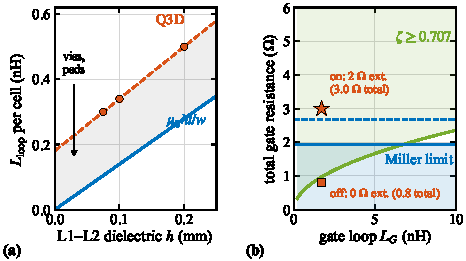
\includegraphics[width=\linewidth]{fig_parasitics.pdf}
\column{0.53\textwidth}
\small
\begin{tabular}{@{}lr@{}}
\toprule
Power loop per cell (copper + ESL) & 0.374\,nH \\
Gate loop $L_G$ per transistor & 1.71\,nH \\
$L_{CS}$, Kelvin / no Kelvin & 0.030 / 0.061\,nH \\
Gate loop -- gate loop mutual & 0.46\,nH \\
Busbar, leg to leg (1\,MHz) & 3.35\,nH \\
Busbar, series tab to leg & 41\,nH \\
\bottomrule
\end{tabular}
\vspace{1ex}

\footnotesize Busbar: DC$+$ and DC$-$ tabs leave at opposite ends (41\,nH); bring them out together or use a laminated cell interconnect.
\end{columns}
\end{frame}
\begin{frame}{Switching behaviour}
\centering
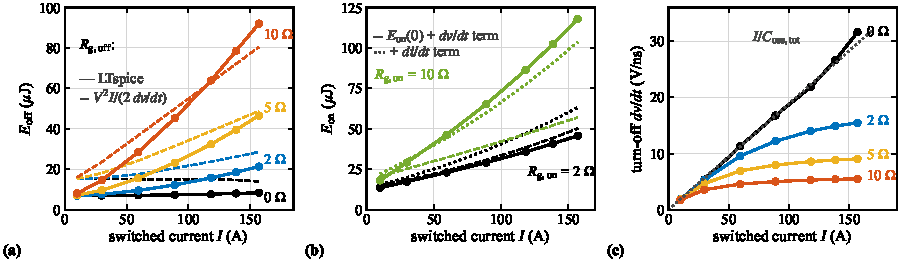
\includegraphics[width=\linewidth,height=0.72\textheight,keepaspectratio]{fig_switching.pdf}
\small LTspice with the Q3D power loop and gate star, 75\,V, $R_\mathrm{g,on}/R_\mathrm{g,off}$ = 2 / 0\,$\Omega$ external.
\end{frame}
\begin{frame}{Losses and efficiency}
\begin{columns}[T]
\column{0.6\textwidth}
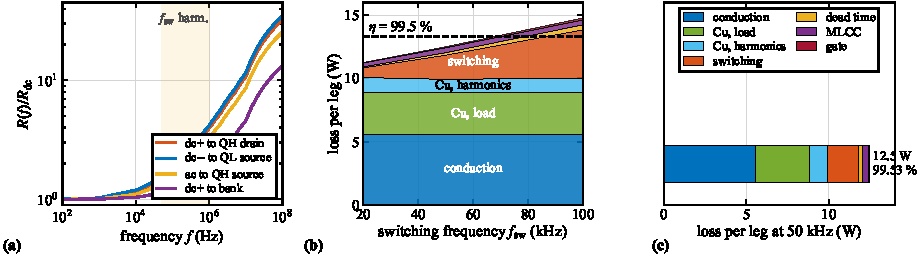
\includegraphics[width=\linewidth]{fig_losses.pdf}
\column{0.38\textwidth}
\small
\begin{itemize}
\item Rated point (75\,V, 100\,A$_\mathrm{rms}$, 50\,kHz): \textbf{12.5\,W per block}, $\eta$ = 99.53\,\%
\item At 300\,kW ($\cos\varphi$ = 0.9) the block carries 114\,A$_\mathrm{rms}$: see the block summary slide
\item Worst case 14.3\,W (99.46\,\%)
\item 1.91\,W per transistor
\item Copper and switching harmonics add $\approx$\,1/3 to the DC copper loss
\end{itemize}
\end{columns}
\end{frame}
\begin{frame}{Thermal design}
\begin{columns}[T]
\column{0.6\textwidth}
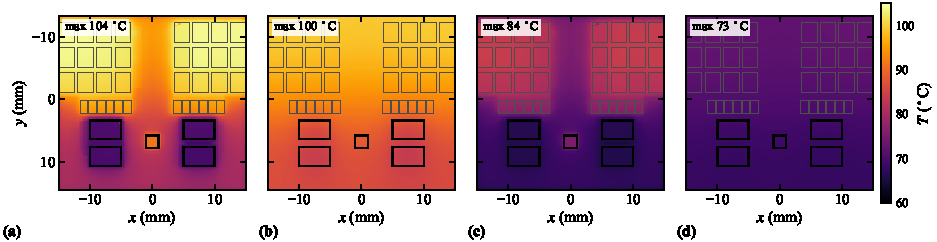
\includegraphics[width=\linewidth]{fig_thermal.pdf}
\column{0.38\textwidth}
\small
\begin{itemize}
\item Top-side cooling through an insulating interface to a liquid cold plate (integration concept)
\item Icepak: $T_j \approx 64\,^\circ$C at the rated point
\item Lab: fan heatsink on the Rev A board (later slide)
\end{itemize}
\end{columns}
\end{frame}
\begin{frame}{Gate bump at the high side}
\begin{columns}[T]
\column{0.58\textwidth}
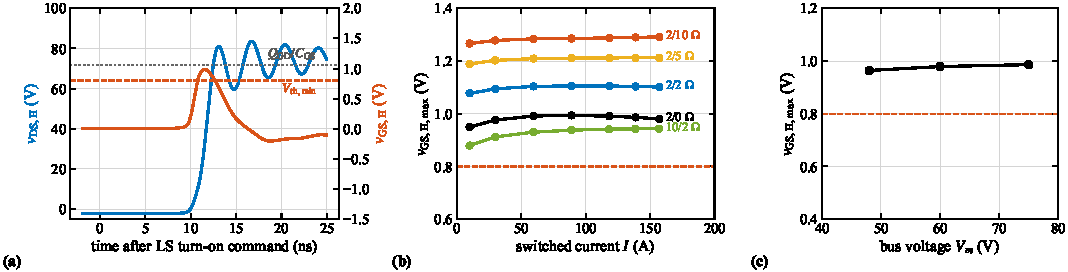
\includegraphics[width=\linewidth]{bump_mechanism.pdf}
\column{0.4\textwidth}
\small
\begin{itemize}
\item When the low side turns on, the high-side drain sees $dv/dt$: Miller charge flows into $C_{GS}$
\item Bump $\approx Q_{GD}/C_{GS} \approx 1.06$\,V, $\approx$\,2\,ns, \textbf{independent of current and voltage}
\item Below the 1.1\,V typical threshold, close to the 0.8\,V minimum: no shoot-through in simulation, but little margin
\end{itemize}
\end{columns}
\end{frame}
\begin{frame}{Mitigation: negative off-voltage}
\begin{columns}[T]
\column{0.58\textwidth}
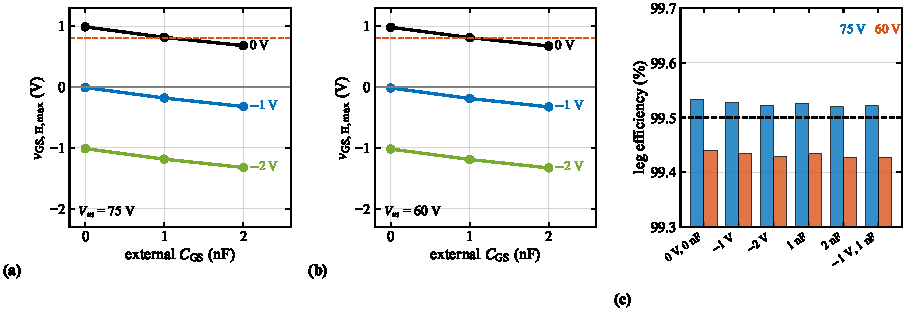
\includegraphics[width=\linewidth]{bump_mitigation.pdf}
\column{0.4\textwidth}
\small
\begin{itemize}
\item With $-1$\,V off-voltage the peak falls from 0.99\,V to $-0.01$\,V
\item Undershoot $-2.3$\,V, rating $-4$\,V
\item Cost: reverse conduction drop in the dead time rises by 1\,V
\item Dead-time loss 0.20 / 0.29 / 0.38\,W per leg for 0 / $-1$ / $-2$\,V
\item \textbf{Chosen: $\approx -1.24$\,V}
\end{itemize}
\end{columns}
\end{frame}
\begin{frame}{Driver: Infineon 2EDF7275K}
\begin{columns}[T]
\column{0.58\textwidth}
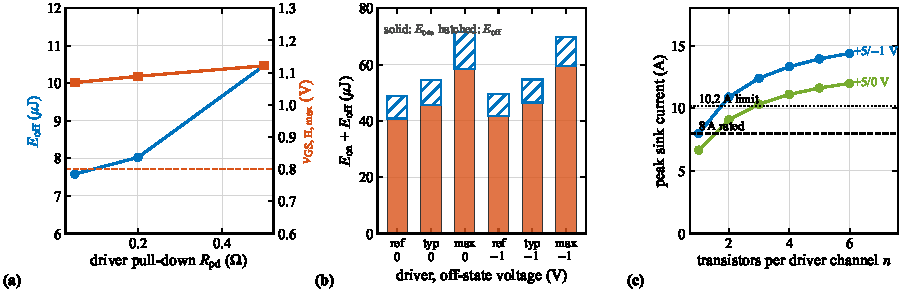
\includegraphics[width=\linewidth]{drv_output_stage.pdf}
\column{0.4\textwidth}
\small
\begin{itemize}
\item Dual isolated channel, 4\,A source / 8\,A sink, 0.85 / 0.35\,$\Omega$
\item 4\,V UVLO: allows a split $+5/-1.24$\,V supply per channel
\item Sink strength sets the turn-off ($E_\mathrm{off}$), not the bump
\item LGA-13, 5\,$\times$\,5\,mm; functional isolation only
\end{itemize}
\end{columns}
\end{frame}
\begin{frame}{Negative rail vs dead-time loss}
\centering
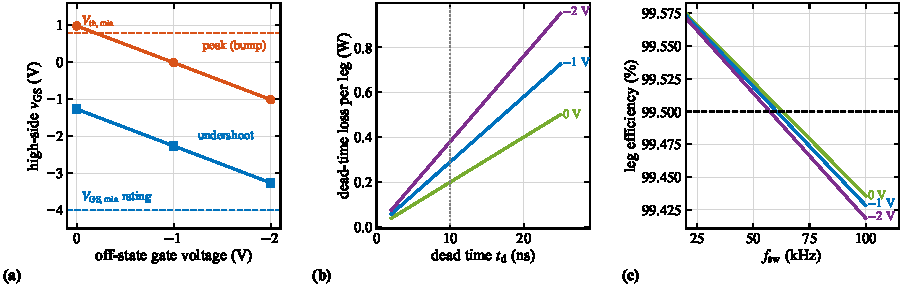
\includegraphics[width=\linewidth,height=0.75\textheight,keepaspectratio]{drv_negative_rail.pdf}
\end{frame}
\begin{frame}{Machine-integrated drive concept}
\begin{columns}[T]
\column{0.55\textwidth}
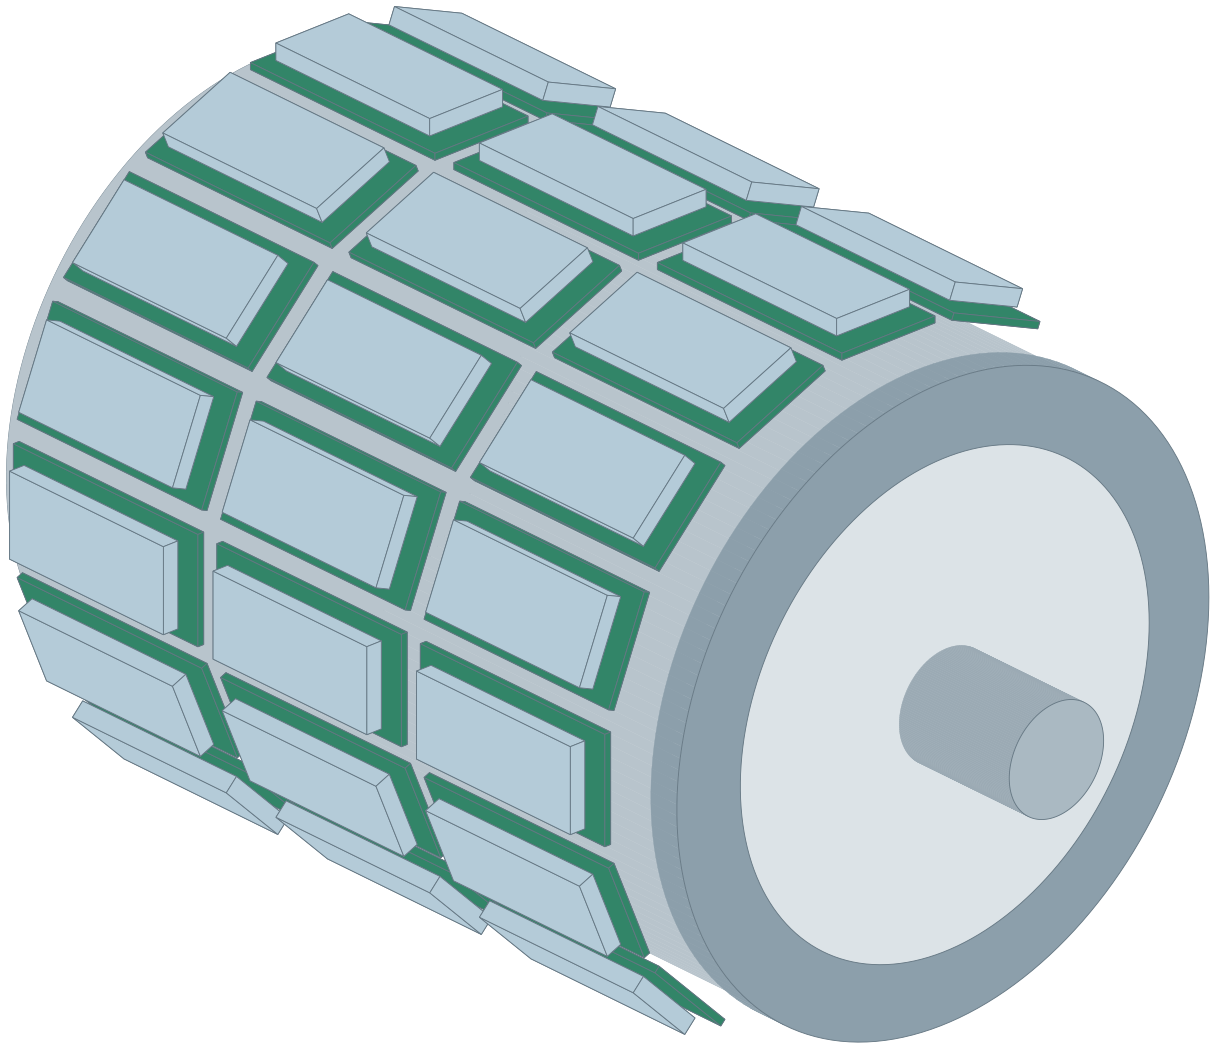
\includegraphics[width=\linewidth]{motor_integration.png}
\column{0.43\textwidth}
\small
\begin{itemize}
\item One submodule = one cell assembly on a liquid cold plate (AlN insulation); at 300\,kW six blocks (3 legs $\times$ 2)
\item Laminated busbar along the cells, phase leads to the winding sets
\item Machine side feeds back into $N$ (winding sets) and $f_\mathrm{sw}$ (ripple, iron loss)
\end{itemize}
\end{columns}
\end{frame}
\begin{frame}{Cell assembly and busbar}
\begin{columns}[T]
\column{0.5\textwidth}
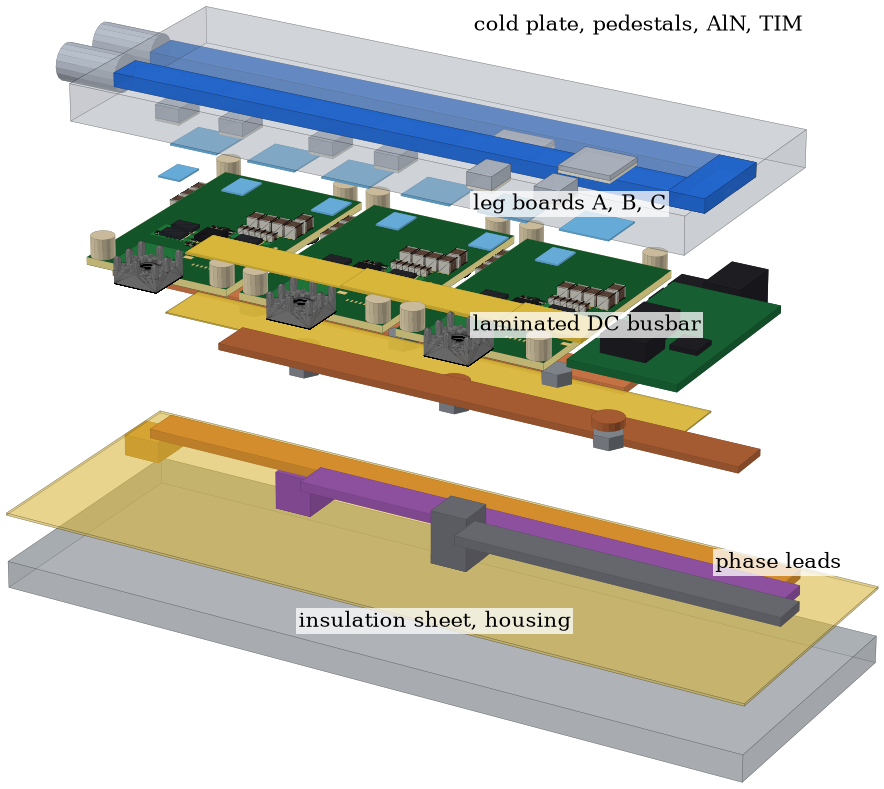
\includegraphics[width=\linewidth]{cell_exploded.png}
\column{0.48\textwidth}
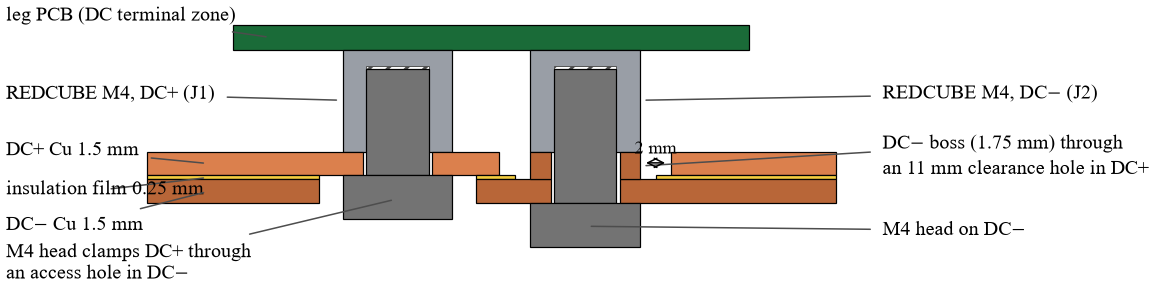
\includegraphics[width=\linewidth]{busbar_section.png}
\small
\begin{itemize}
\item Leg-to-leg busbar inductance 3.35\,nH (Q3D)
\item Series tabs: 41\,nH because DC$+$ and DC$-$ leave at opposite ends
\end{itemize}
\end{columns}
\end{frame}
%==================================================================== 9
\section{10\quad Rev A fabrication board}
\begin{frame}{Rev A board: overview}
\begin{columns}[T]
\column{0.6\textwidth}
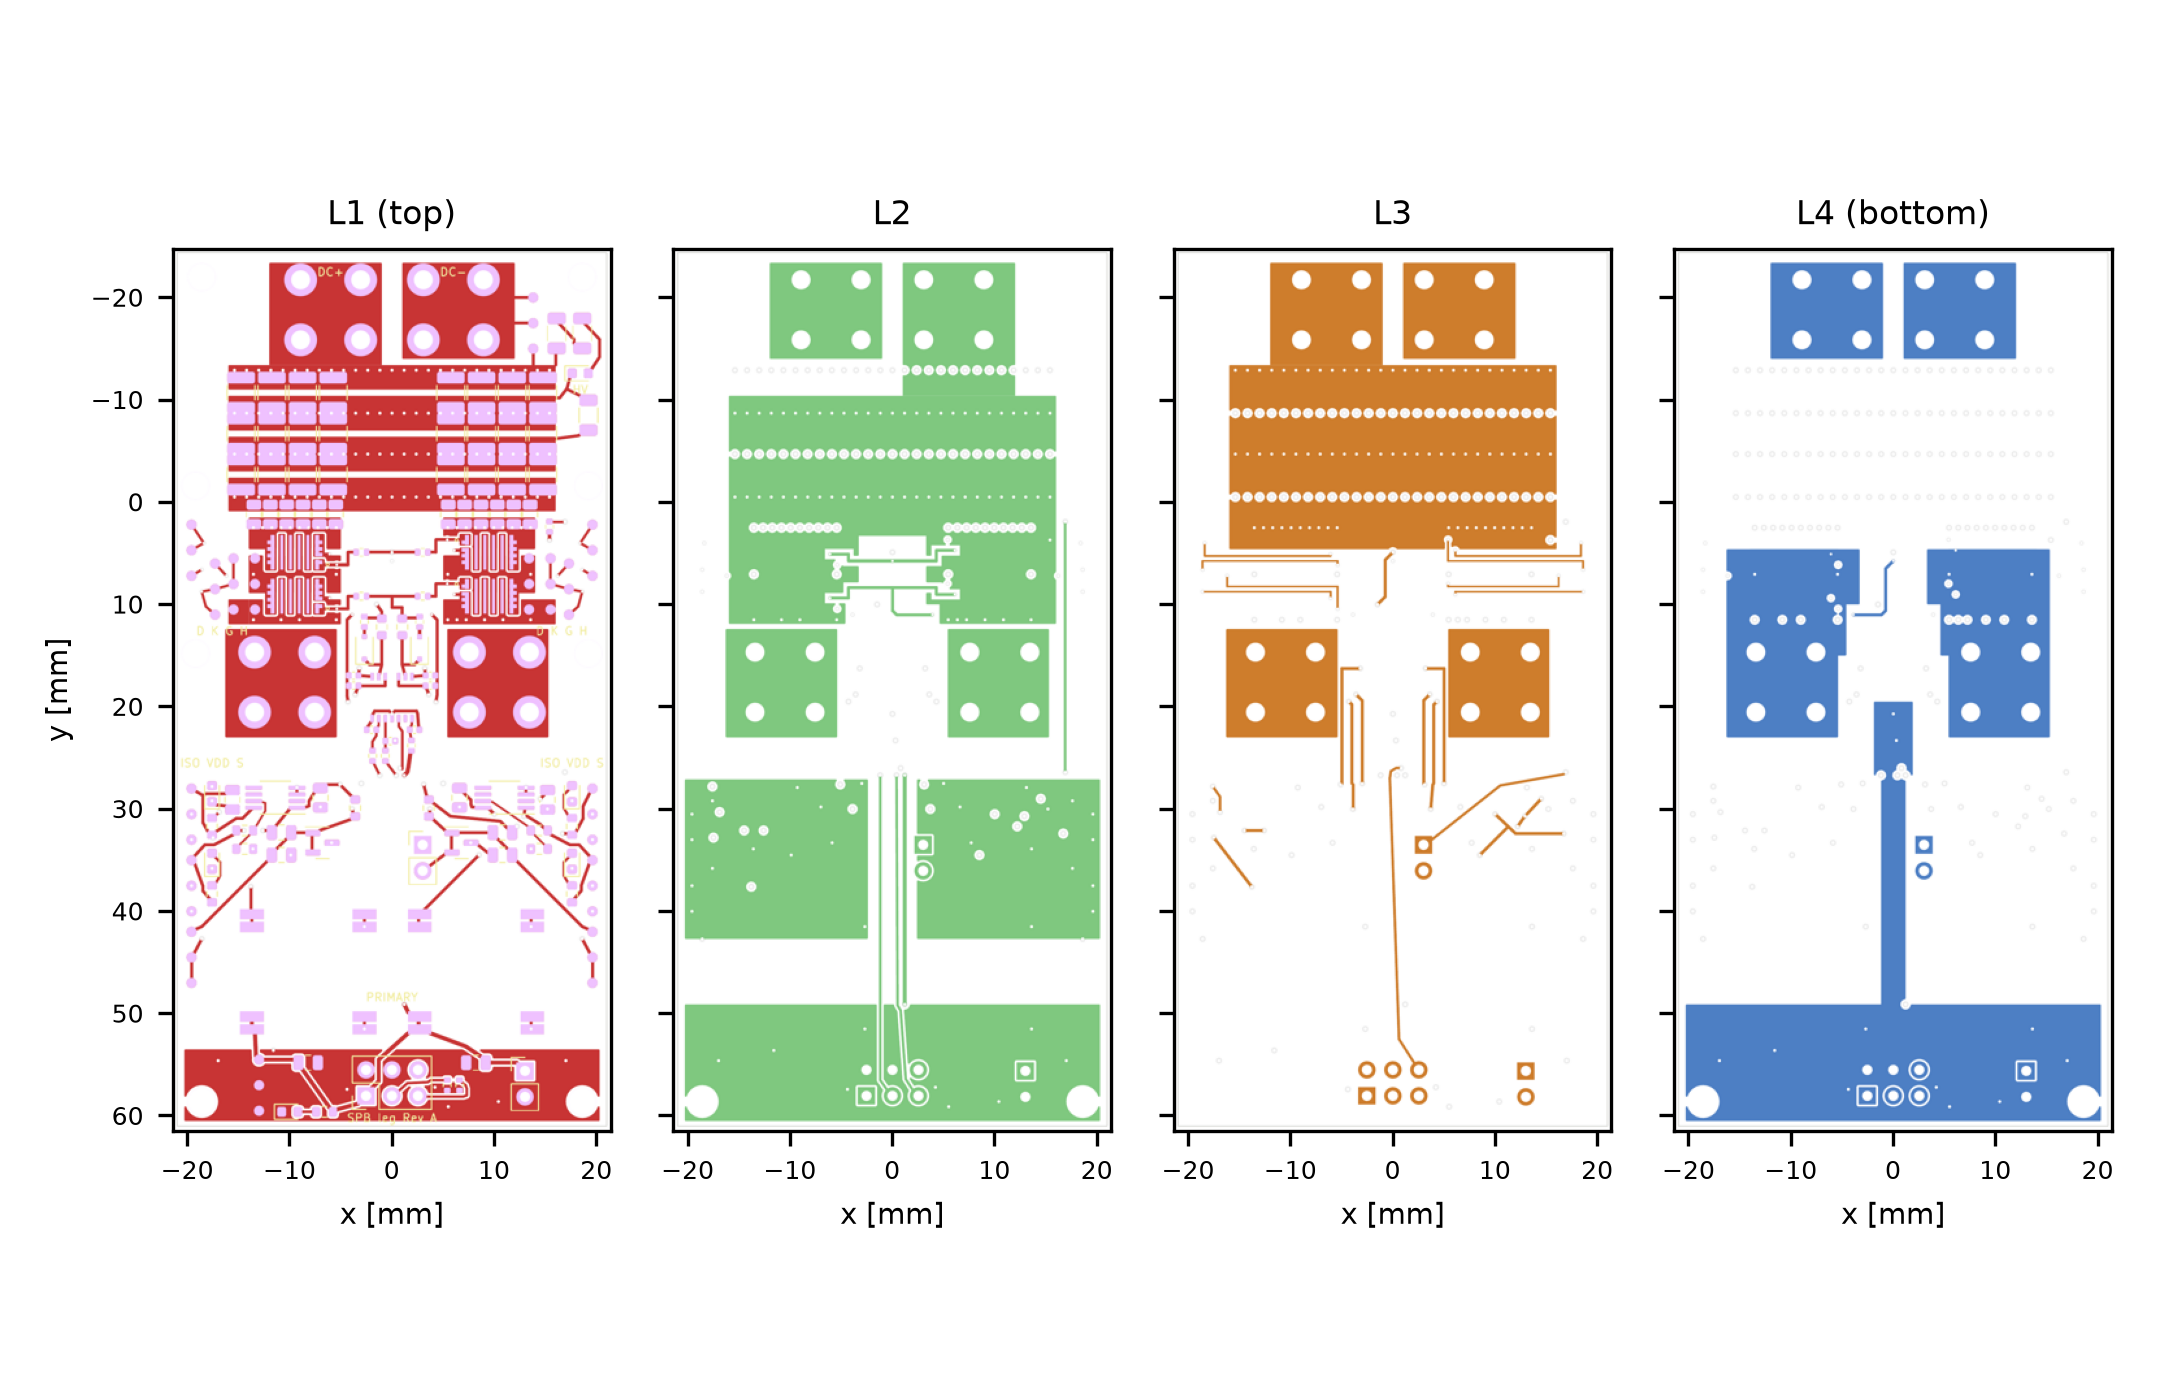
\includegraphics[width=\linewidth]{fig_layers.png}
\column{0.38\textwidth}
\small
\begin{itemize}
\item 42\,$\times$\,85.4\,mm, 4 layers, 4\,$\times$\,70\,\textmu m
\item DC terminals (top), two cells, driver corridor, AC terminals below each switch node, gate supplies, primary side (bottom)
\item Outer strips: heatsink holes, probe landings, LEDs
\item Fully scripted (KiCad~7 Python), DRC 0 / 0, wired schematic identical netlist
\end{itemize}
\end{columns}
\end{frame}
\begin{frame}{Stack-up and design rules}
\small
\begin{tabularx}{\linewidth}{@{}llX@{}}
\toprule
L1 70\,\textmu m & power, pads, gate stars & all components \\
prepreg 0.1\,mm & & vertical commutation loop \\
L2 70\,\textmu m & DC$-$ plane & loop return, Kelvin collectors in narrow keepouts \\
core $\approx$\,1.1\,mm & & \\
L3 70\,\textmu m & DC$+$ plane & HS gate trunk, supply columns, probe sense pairs \\
prepreg 0.1\,mm & & HS gate trunk over its Kelvin return \\
L4 70\,\textmu m & AC plane & switch node to J3/J4, HS Kelvin return, primary ground \\
\midrule
Rules & 0.15/0.15\,mm & power gaps 0.2\,mm under solder mask (IPC-2221B B4: 0.13\,mm for 51--100\,V) \\
Vias & 0.6/0.3\,mm, 0.45/0.25\,mm & no via-in-pad, standard process \\
\bottomrule
\end{tabularx}
\end{frame}
\begin{frame}{Gate loops in the driver corridor}
\centering
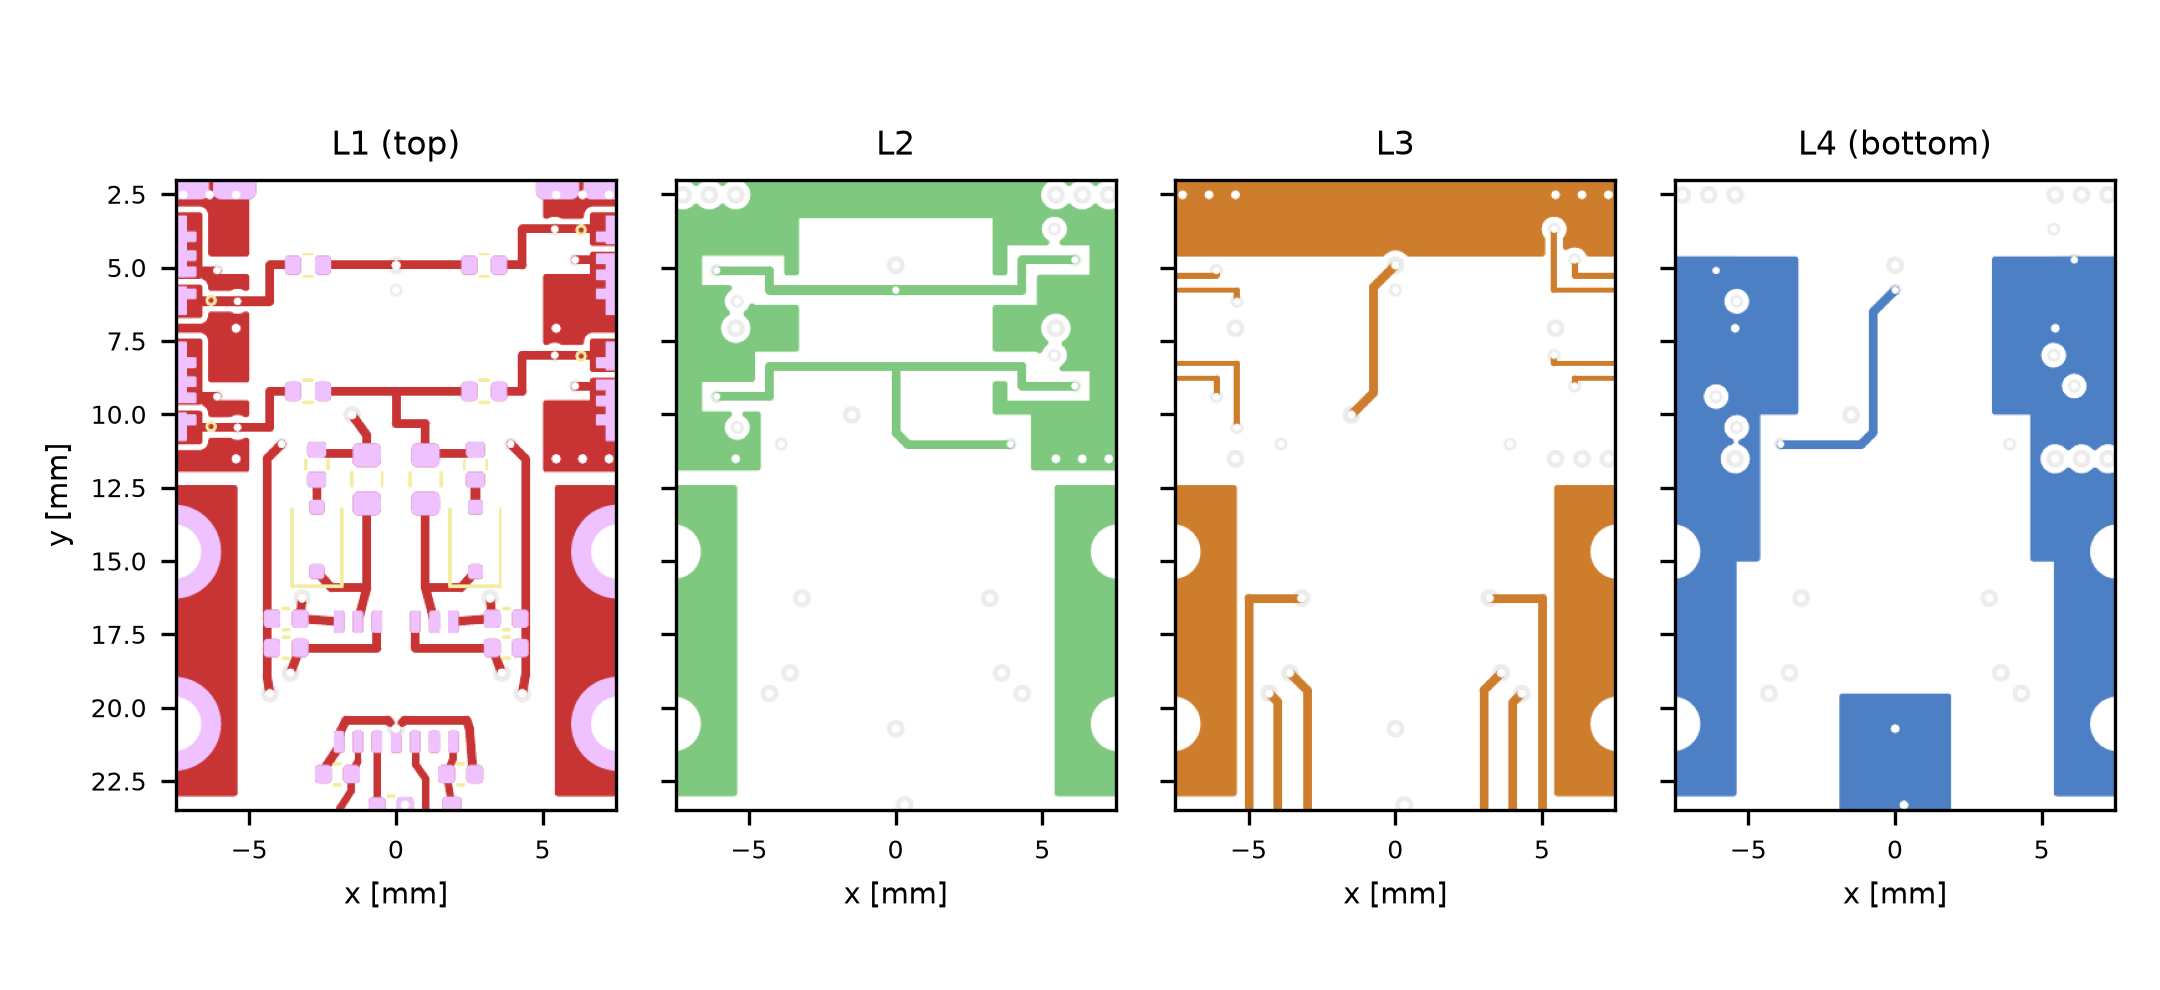
\includegraphics[width=\linewidth,height=0.62\textheight,keepaspectratio]{fig_corridor.png}
\small
\begin{itemize}
\item HS: trunk on L3, Kelvin return directly below on L4; LS: star on L1, Kelvin collector on L2
\item Kelvin collectors join on the symmetry line $\Rightarrow$ identical gate loops for both transistors
\end{itemize}
\end{frame}
\begin{frame}{Separate turn-on and turn-off paths}
\begin{columns}[T]
\column{0.5\textwidth}
\centering
\begin{circuitikz}[scale=0.8,transform shape]
\draw (0,0) node[left]{OUT} to[short,o-*] (1,0) to[R,l=$R_\mathrm{ON}$] (4,0) to[short,-*] (5,0);
\draw (1,0) -- (1,-1.5) to[D*,l_=$D$,invert] (2.6,-1.5) to[R,l_=$R_\mathrm{OFF}$] (4.6,-1.5) -- (5,-1.5) -- (5,0);
\draw (5,0) to[short] (5.6,0) node[right]{trunk / star};
\draw (5.6,0) -- (5.6,1) to[R,l=$R_{G,1}$] (8,1) node[right]{G$_1$};
\draw (5.6,0) -- (5.6,-1) to[R,l_=$R_{G,2}$] (8,-1) node[right]{G$_2$};
\draw (5.6,0) to[short,*-] (5.6,0);
\end{circuitikz}
\vspace{1ex}

\small $R_\mathrm{on,eff} = 2R_\mathrm{ON}+R_{G,i}$\\
$R_\mathrm{off,eff} \approx 2(R_\mathrm{ON}\parallel R_\mathrm{OFF})+R_{G,i}\;(+V_F)$
\column{0.48\textwidth}
\small
\begin{tabular}{@{}lll@{}}
\toprule
Part & default & per transistor \\
\midrule
$R_\mathrm{ON}$ (0603) & 0.75\,$\Omega$ & on: 2.0\,$\Omega$ \\
$R_\mathrm{OFF}$ (0402) & 0\,$\Omega$ & off: 0.5\,$\Omega$ + D \\
D PMEG3020EJ & SOD323F & \\
$R_{G,i}$ (0402) & 0.5\,$\Omega$ & \\
\bottomrule
\end{tabular}
\begin{itemize}
\item Peak gate current 3.1\,A (on) / 6.5\,A (off): within 4 / 8\,A
\item Same as the simulated 2\,$\Omega$ / 0\,$\Omega$ external
\item Values changeable by population
\item 10\,k$\Omega$ pull-down star $\rightarrow$ Kelvin per switch
\end{itemize}
\end{columns}
\end{frame}
\begin{frame}{Driver schematic (KiCad)}
\centering
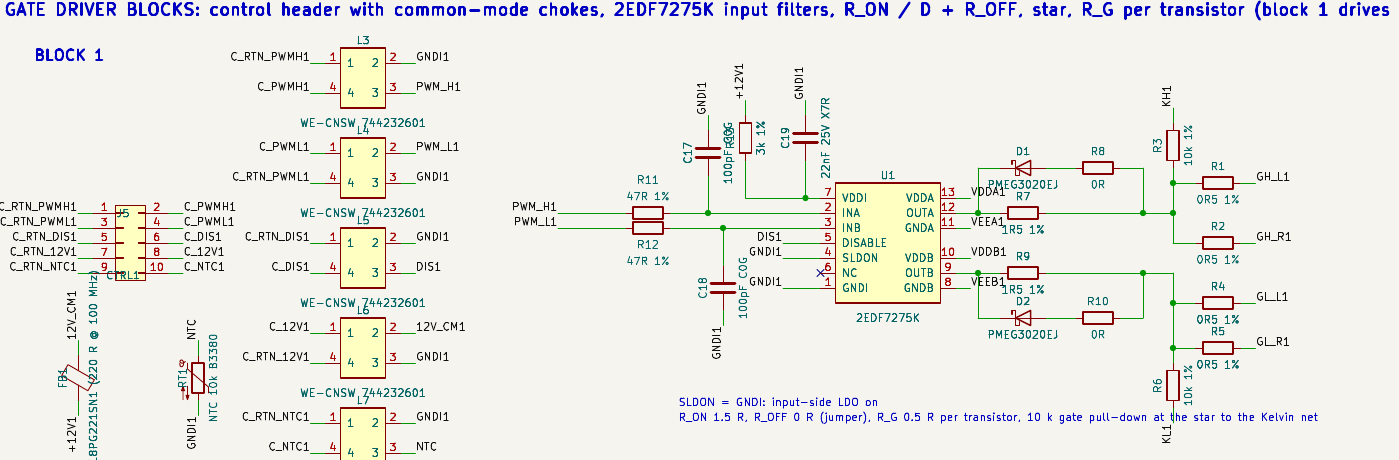
\includegraphics[width=\linewidth,height=0.8\textheight,keepaspectratio]{sch_driver.png}
\end{frame}
\begin{frame}{Isolated gate supplies}
\begin{columns}[T]
\column{0.5\textwidth}
\centering
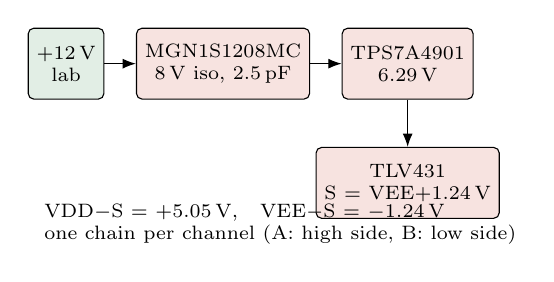
\begin{tikzpicture}[font=\scriptsize,node distance=4mm,
  b/.style={draw,rounded corners=2pt,minimum height=9mm,align=center,inner sep=3pt}]
\node[b,fill=pri!15] (p) {+12\,V\\lab};
\node[b,fill=hs!15,right=of p] (m) {MGN1S1208MC\\8\,V iso, 2.5\,pF};
\node[b,fill=hs!15,right=of m] (l) {TPS7A4901\\6.29\,V};
\node[b,fill=hs!15,below=6mm of l] (t) {TLV431\\S = VEE+1.24\,V};
\draw[-{Latex}] (p) -- (m); \draw[-{Latex}] (m) -- (l); \draw[-{Latex}] (l) -- (t);
\node[below=12mm of p,anchor=north west,align=left,xshift=-4mm] {VDD$-$S = +5.05\,V,\quad VEE$-$S = $-1.24$\,V\\one chain per channel (A: high side, B: low side)};
\end{tikzpicture}
\column{0.48\textwidth}
\small
\begin{itemize}
\item Two isolated supplies: HS reference = switch node, LS reference = DC$-$ (floats up to 1.2\,kV in the stack)
\item TPS7A4901 replaces LP2951: LP2951 has no VSSOP and its legacy chip needs ESR $\geq$\,30\,m$\Omega$
\item $V_\mathrm{OUT} = 1.185\,\mathrm{V}\,(1+102\,\mathrm{k}/23.7\,\mathrm{k})$; stable with ceramics $\geq$\,2.2\,\textmu F
\item TLV431 stable: $>$\,5\,\textmu F on S$-$VEE (unstable band 0.02--0.8\,\textmu F)
\item Budget per channel at 50\,kHz: 65\,nC, 7.6\,mA, 61\,mW
\end{itemize}
\end{columns}
\end{frame}
\begin{frame}{Supply schematic (KiCad)}
\centering
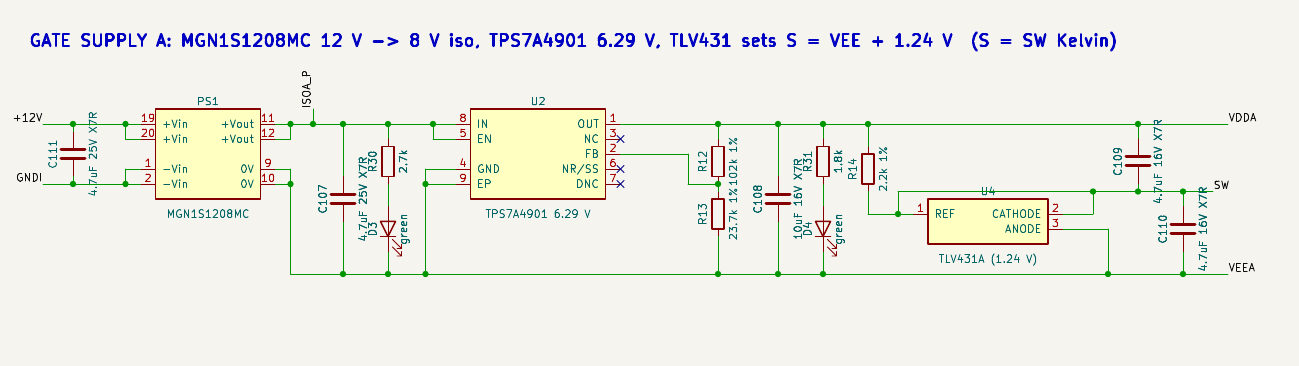
\includegraphics[width=\linewidth,height=0.8\textheight,keepaspectratio]{sch_supply.png}
\end{frame}
\begin{frame}{Isolation domains}
\begin{columns}[T]
\column{0.5\textwidth}
\small
\begin{tabular}{@{}lrr@{}}
\toprule
Domains & outer & inner \\
\midrule
DC$+$ -- switch node & 0.20 & 0.65 \\
DC$+$ -- DC$-$ & 0.70 & 1.07 \\
HS -- LS & 0.20 & 0.40 \\
HS -- primary & 1.37 & 1.08 \\
LS -- primary & 1.50 & 0.75 \\
\bottomrule
\end{tabular}
{\scriptsize minimum copper spacing [mm] on the routed board}
\column{0.48\textwidth}
\small
\begin{itemize}
\item Power domains $\leq$\,100\,V: 0.2\,mm under mask
\item Primary side separated functionally (lab board)
\item In the 1200\,V stack: PWM via fibre / reinforced isolator and isolated 12\,V at the controller side; 2EDF7275K is functional only
\end{itemize}
\end{columns}
\end{frame}
\begin{frame}{Double-pulse test: measurement landings}
\begin{columns}[T]
\column{0.55\textwidth}
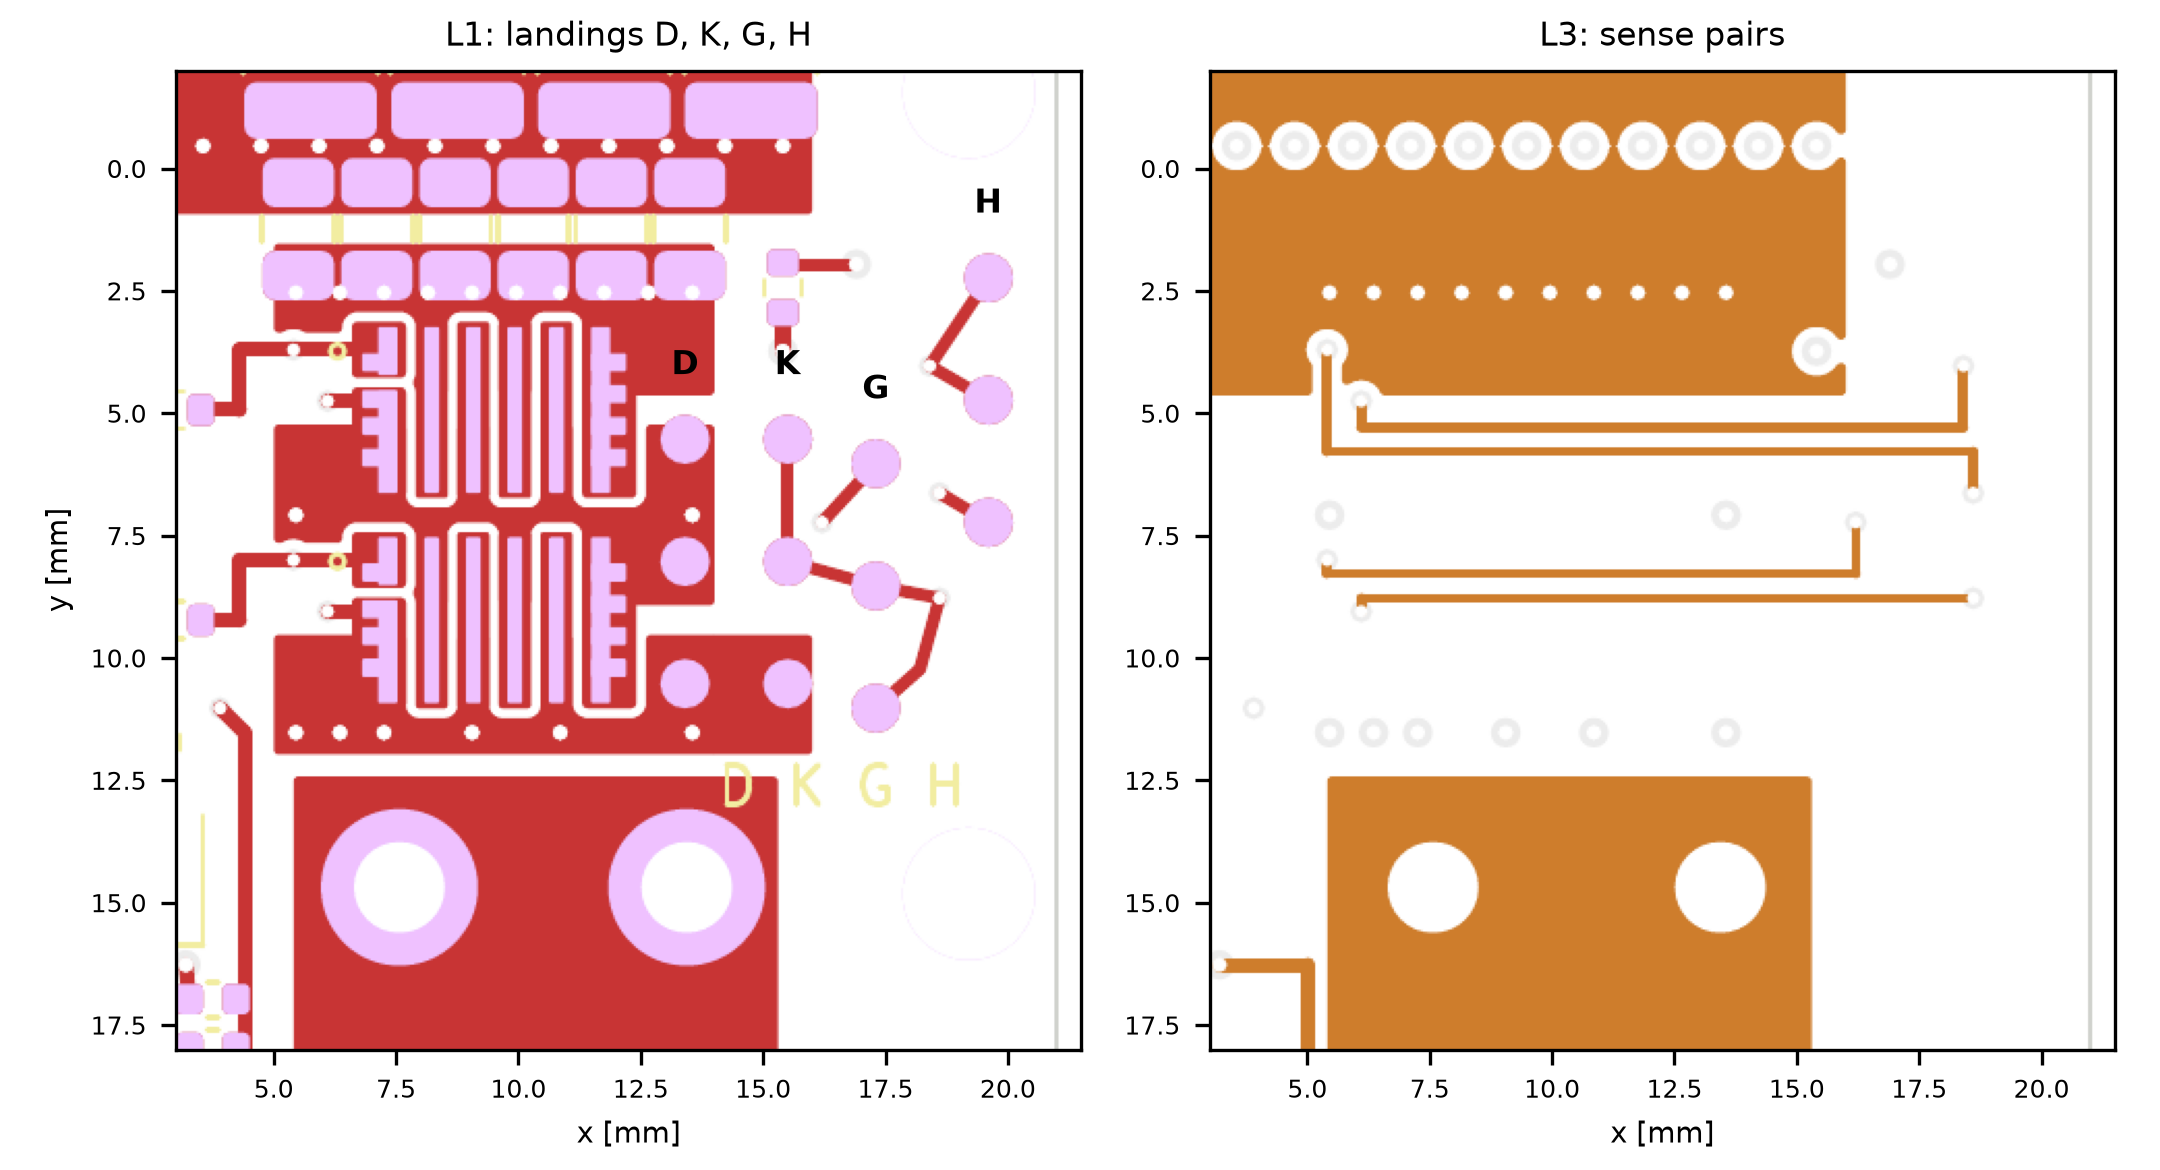
\includegraphics[width=\linewidth]{fig_landings.png}
\column{0.43\textwidth}
\small
\begin{itemize}
\item Probe pads only, outside the commutation loop; spring ground at 2.5 and 5.0\,mm
\item \textbf{D}: $V_{DS}$ of Q3 / Q4 at the package
\item \textbf{K}: $v_{KS}$ = Kelvin vs power-source copper
\item \textbf{G}: $V_{GS}$ of Q3 / Q4 (sense pairs on L3)
\item \textbf{H}: $V_{GS}$ of Q1 / Q2 (isolated probe)
\item Inductor current: Rogowski / Pearson off the board
\end{itemize}
\end{columns}
\end{frame}
\begin{frame}{$E_\mathrm{on}$, $E_\mathrm{off}$ and per-transistor current}
\small
\begin{itemize}
\item $E = \int v_{DS}\, i_D\, dt$; $E_\mathrm{off}$ with $i_D = I_L$; $E_\mathrm{on}$ with $I_L$ plus the high-side output charge $Q_\mathrm{OSS}V_\mathrm{DC}$
\item Deskew $<$\,50\,ps: 100\,ps at 50\,V/ns and 100\,A $\approx$ 0.75\,\textmu J error ($\approx$\,8\,\% of $E_\mathrm{on}$)
\item Per-transistor current without a shunt (no extra loop inductance):
\[ v_{KS} = L_s\,\frac{di_D}{dt} + R_s i_D \quad\Rightarrow\quad \Delta i_D(t) \approx \frac{1}{L_s}\int v_{KS}\,dt \]
$L_s \approx 0.03$\,nH: $\approx$\,0.5\,V at 17\,A/ns; scale with $i_3+i_4 = I_L$, ratio gives the dynamic sharing
\item Same principle as stray-inductance di/dt sensing in SiC short-circuit protection (Sun, CPES 2019; Xue et al., TPEL 2020)
\item Rogowski holes in the cells: not possible without opening the L1/L2 loop; coil bandwidth (20--50\,MHz) too low for 2--3\,ns edges
\end{itemize}
\end{frame}
\begin{frame}{Bring-up: test points, LEDs, protection}
\begin{columns}[T]
\column{0.55\textwidth}
\scriptsize
\begin{tabular}{@{}lll@{}}
\toprule
Item & nets & expected \\
\midrule
TP15, D7 & +12\,V & 12\,V present \\
TP9/12, D3/5 & ISO / VEE & MGN1 output 8--10\,V \\
TP10/13, D4/6 & VDD / VEE & 6.29\,V \\
TP11/14 & S / VEE & 1.24\,V \\
TP16, D8 (red) & DC link & charged; 100\,k bleeder \\
R35/R36 & PWM & 10\,k pull-downs \\
R41/R42 & star--Kelvin & 10\,k gate pull-downs \\
J7 & +12\,V & fan \\
\bottomrule
\end{tabular}
\column{0.43\textwidth}
\small
\textbf{Power-up order}
\begin{enumerate}\footnotesize
\item 12\,V (current limit), LEDs on, TP values
\item PWM without DC link: driver outputs on R5/R7, gates on R1--R4
\item DC link 12 $\rightarrow$ 24 $\rightarrow$ 48 $\rightarrow$ 75\,V, double-pulse test
\item Heatsink, continuous operation
\end{enumerate}
\footnotesize Power down in reverse: DC link first, then 12\,V.
\end{columns}
\end{frame}
\begin{frame}{Cooling for the load test}
\begin{columns}[T]
\column{0.55\textwidth}
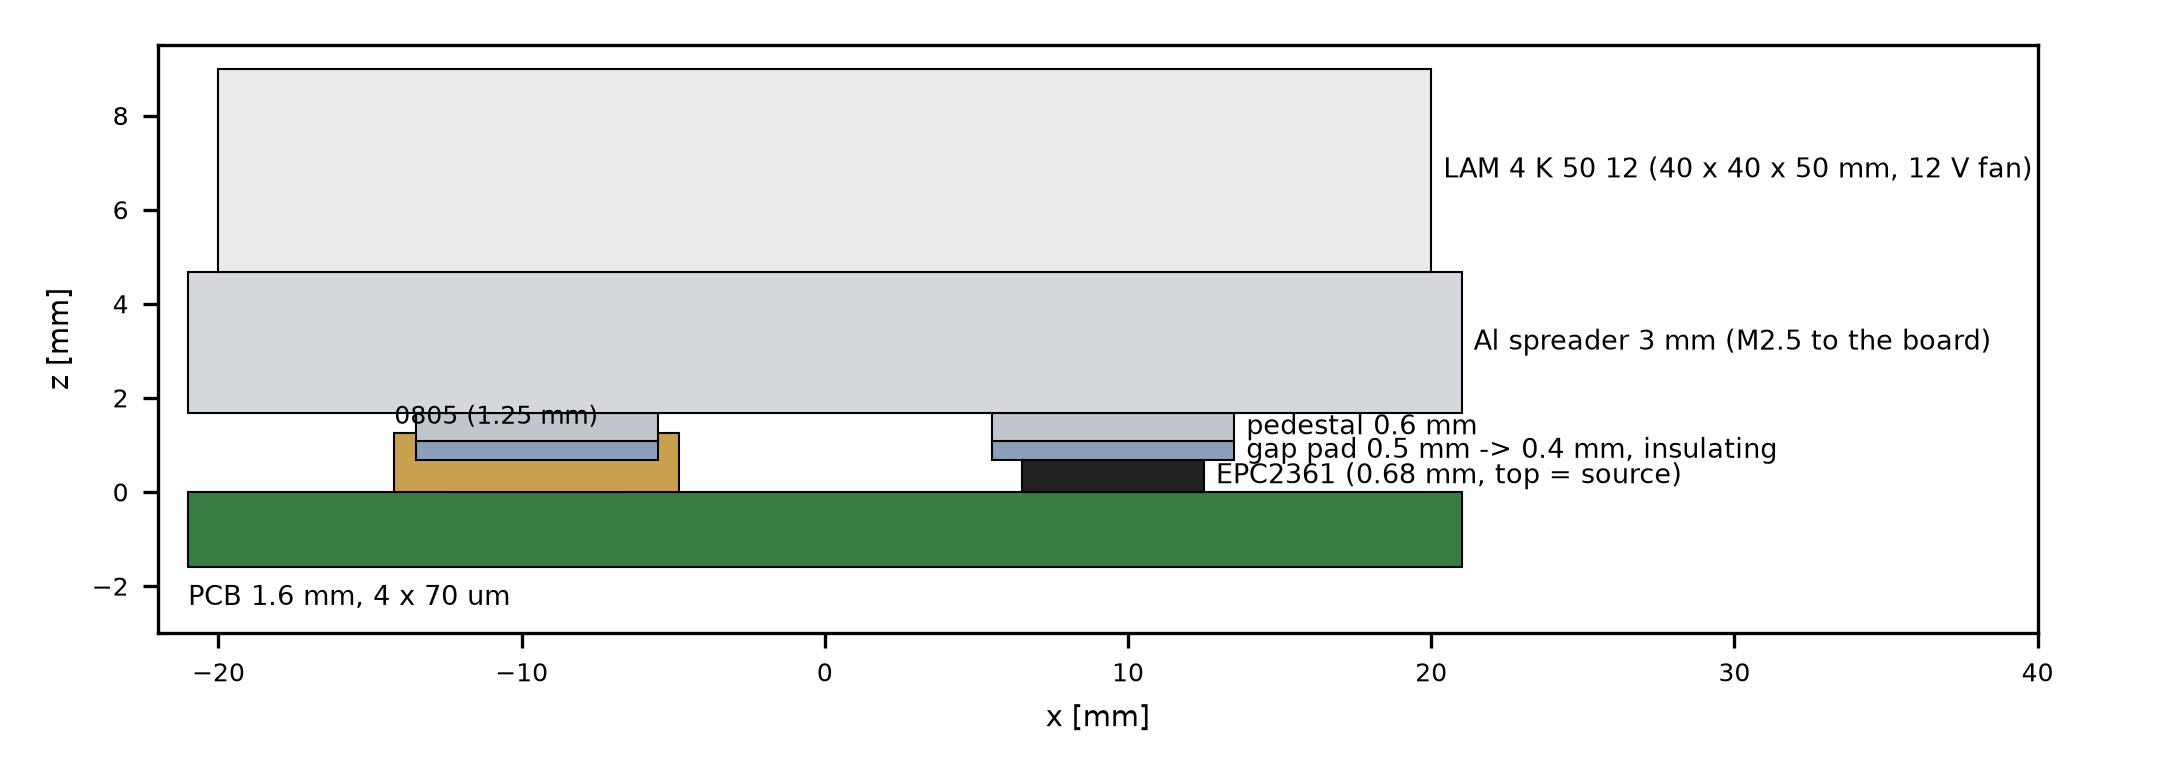
\includegraphics[width=\linewidth]{fig_heatsink.png}
\column{0.43\textwidth}
\small
\begin{itemize}
\item Fischer LAM 4 K 50 12 (0.65\,K/W, 12\,V fan from J7), off the shelf
\item Al spreader 42\,$\times$\,14\,$\times$\,3\,mm (workshop part), 4\,$\times$ M2.5
\item Insulating gap pad 0.5\,mm, $\geq$\,5\,W/mK: 5.3\,K/W per transistor (dominant)
\item $T_j \approx 57\,^\circ$C (40\,$^\circ$C ambient); flat plate + 1\,mm pad: $\approx$\,70\,$^\circ$C
\item Next step: AlN insulator ($\approx$\,1\,K/W per transistor)
\end{itemize}
\end{columns}
\end{frame}
\begin{frame}{Power-stage schematic (KiCad)}
\centering
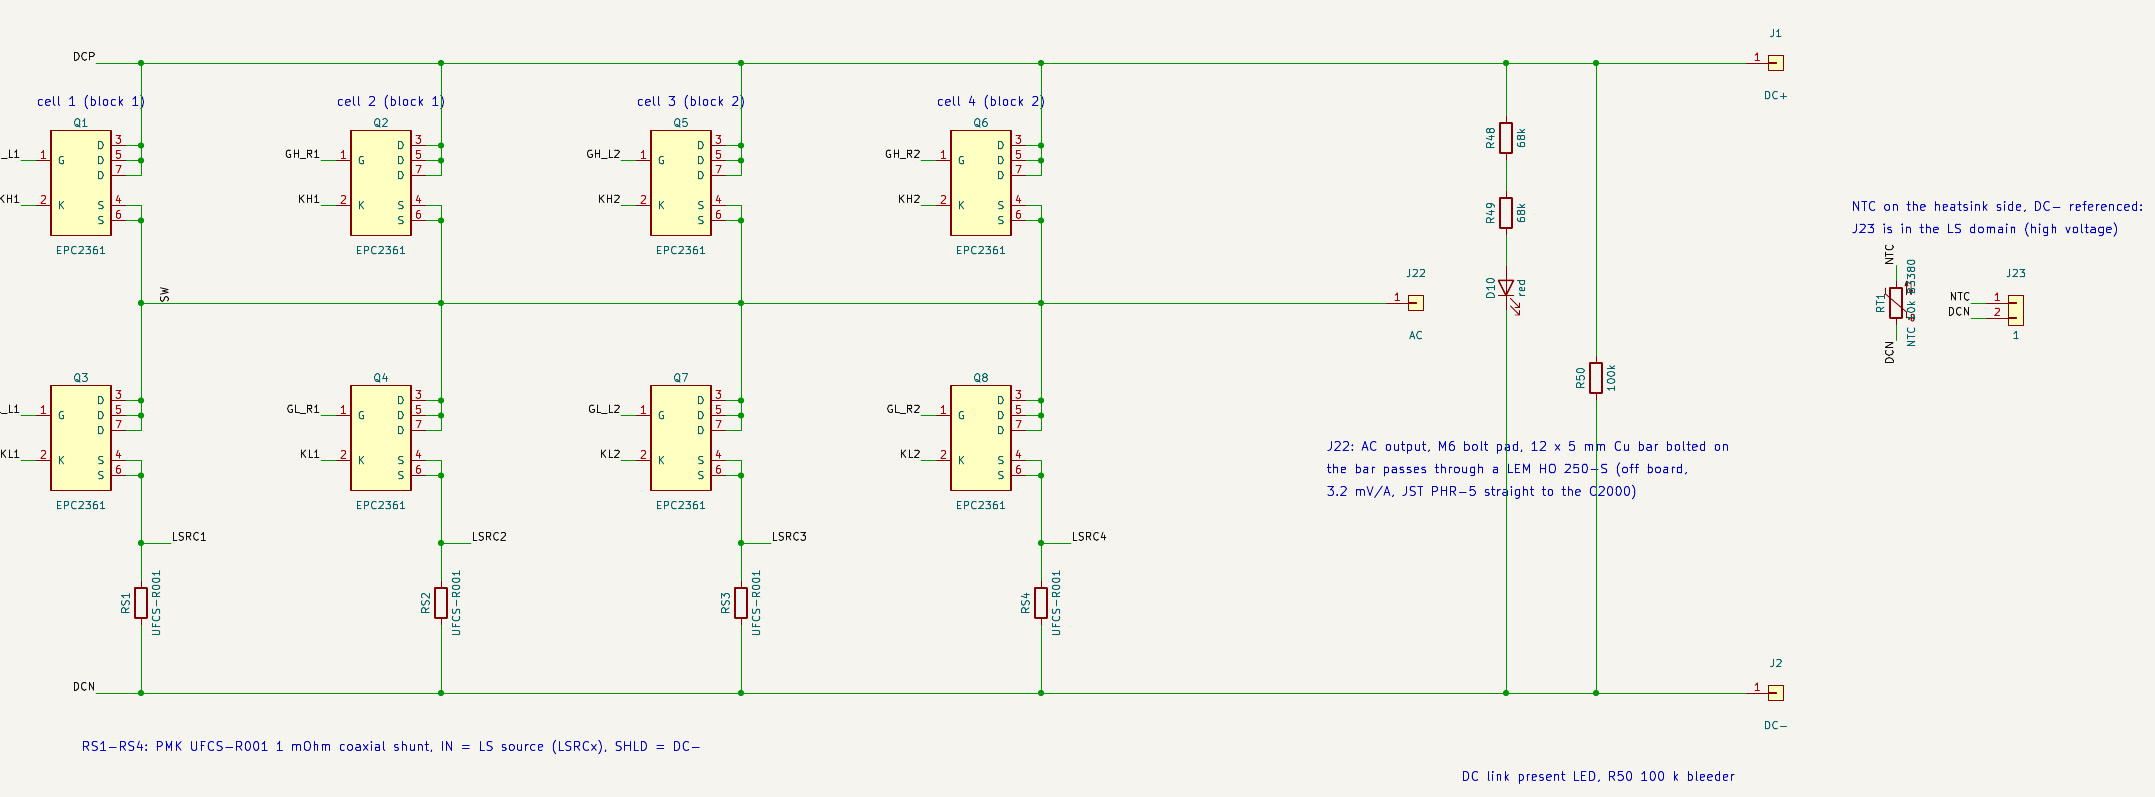
\includegraphics[width=\linewidth,height=0.8\textheight,keepaspectratio]{sch_power.png}
\end{frame}
\section{Status and next steps}
\begin{frame}{Verification status}
\small
\begin{tabularx}{\linewidth}{@{}lX@{}}
\toprule
Done & DRC 0 violations / 0 unconnected; wired schematic = PCB netlist (37 nets); 3D models for all parts, STEP export; Gerber, drill, pick-and-place, BOM (35 lines, 109 parts + mechanics); datasheet checks: TPS7A4901 pins/stability, TLV431 pinout and stability, PMEG3020EJ; spreader drawing; gap pad proposed (Bergquist TGP\,5000, 0.5\,mm) \\
Prepared & Q3D re-extraction of the routed copper (\texttt{run\_bb\_q3d\_fab.cmd}); needs the KTH licence (campus / VPN) \\
Open & Q3D result vs 0.374\,nH design value; gap-pad breakdown rating; fab-house review of 0.2\,mm gaps; isolation concept for the 1200\,V stack; two-block parallel connection (AC/DC interconnect, PWM fan-out) \\
\bottomrule
\end{tabularx}
\end{frame}
\begin{frame}{Next steps}
\begin{enumerate}
\item Re-extract the routed board in Q3D, update loop and gate-loop values
\item Order Rev A, assemble, bring-up (12\,V, PWM, then DC link)
\item Double-pulse test at 12--75\,V: $E_\mathrm{on}$, $E_\mathrm{off}$, gate bump, sharing (D, G, K, H landings)
\item Continuous operation with the fan heatsink; thermal camera
\item Two blocks in parallel (300\,kW leg): double-pulse and continuous test, block-to-block sharing with a Rogowski on each AC lead
\item Compare with LTspice / Q3D; decide 75\,V vs 60\,V submodules
\item Rev B: cell interconnect with laminated tabs, AlN interface, integration form factor (36\,mm pitch)
\end{enumerate}
\end{frame}
\begin{frame}[standout]
Thank you\\[1ex]
\small Questions?
\end{frame}
\end{document}
